\documentclass{ecnuthesis}
% 模版选项:
% printMode     是否开启打印模式, 若缺省则为关闭, 反之则为开启
% 用法示例
% \documentclass[printMode]{ecnuthesis}   (开启打印模式, 适合双面打印)
% \documentclass{ecnuthesis}              (关闭打印模式, 适合提交电子版)

\ecnuSetup {
% 参数设置
% 允许采用两种方式设置选项:
%   1. style/... = ...
%   2. style = { ... = ... }
% 注意事项:
%   1. 请勿在参数设置中出现空行
%   2. "=" 两侧的空格将被忽略
%   3. "/" 两侧的空格不会被忽略
%   4. 请使用英文逗号 "," 分隔选项
%
% info 类用于输入论文信息
    info = {
        title = {面向移动终端的可穿戴动态心电图的智能监测应用},
        % 中文标题
        %
        titleEN = {Intelligent Monitoring Application of Wearable Dynamic Electrocardiogram for Mobile Terminals},
        % 英文标题
        %
        author = {刘议临},
        % 作者姓名
        %
        studentID = {10195101428},
        % 作者学号
        %
        department = {软件工程学院},
        % 学院名称
        %
        major = {软件工程},
        % 专业名称
        %
        supervisor = {王丽苹},
        % 指导教师姓名
        %
        academicTitle = {副教授},
        % 指导教师职称
        %
        year  = 2023,
        % 论文完成年份
        %
        month = 4,
        % 论文完成月份
        %
        keywords = {\todo{关键词}},
        % 中文关键词
        % 请使用英文逗号 "," 以分隔
        %
        keywordsEN = {\todo{keywords}},
        % 英文关键词
        % 请使用英文逗号 "," 以分隔
        %
    },
% style 类用于简单设置论文格式
    style = {
        footnote  = plain,
        % 脚注编号样式
        % 可用选项:
        %   footnote = plain|circled
        % 说明:
        %   plain     脚注的编号仅为数字
        %   circled   脚注的编号为带圆圈数字 (仅限1-10)
        %   (默认选项为 plain )
        %
        numbering = arabic,
        % 章节编号样式
        % 可用选项:
        %   numbering = arabic|alpha|chinese
        % 说明:
        %   arabic    使用数字进行编号 (即理科要求)
        %   alpha     使用字母进行编号 (即外文要求)
        %   chinese   使用汉字进行编号 (即文科要求)
        %   (默认选项为 arabic )
        %
        fontCJK = fandol,
        % 中文字体选择
        % 可用选项:
        %   fontCJK = fandol|windows|mac
        % 说明:
        %   fandol    使用 TeX 自带的 fandol 字体
        %   windows   使用 Windows 系统内的字体 (中易)
        %   mac       使用 MacOS 系统内的字体
        %   (默认选项为 fandol )
        %
        fontMath = lm,
        % 数学字体选择
        % 可用选项:
        %   fontMath = lm|times
        % 说明:
        %   lm        使用 TeX 自带的 Latin Modern 数学字体
        %   times     使用 Times 风格的数学字体
        %   (默认选项为 lm )
        %
        bibResource = {./thesis-ref.bib},
        % 参考文献数据源
        % 由于使用的是 biber + biblatex , 所以必须明确给出 .bib 后缀名
        %
        logoResource = {./inner-cover(contains-font).eps},
        % 封面插图数据源
        % 模版已自带, 位于 ./inner-cover(contains-font).eps
        % 默认值为空
    }
}

% 需要的宏包可以自行调用
\usepackage[chapter]{easy-todo}
\usepackage{graphicx}
\usepackage{newfloat}
\usepackage{hyperref}
\usepackage{subcaption}
\usepackage{listings}
\usepackage{amsmath}

% https://tex.stackexchange.com/a/584994/254533
\captionsetup[figure][bi-second]{name=Figure}
\captionsetup[bi-second]{listtype+=Eng}
\DeclareFloatingEnvironment[fileext=lof2]{figureEng}[Figure][Figures]

% table
\captionsetup[table][bi-second]{name=Table}
\captionsetup[bi-second]{listtype+=Eng}
\DeclareFloatingEnvironment[fileext=lot2]{tableEng}[Table][Tables]

\newcommand*{\app}{可穿戴动态心电监测应用}

\lstMakeShortInline[columns=fixed]@

\begin{document}

% 设置前置部分编号
    \frontmatter

    % 除了中英文摘要,通常不需要修改其他内容

\clearpage
%\thispagestyle{empty}
\newcommand{\TitleCHS}{面向移动终端的可穿戴动态心电图的智能监测应用} %中文标题

\newcommand{\TitleENG}{Intelligent Monitoring Application of Wearable Dynamic Electrocardiogram for Mobile Terminals} %英文标题

\newcommand{\Author}{刘议临} %作者名字

\newcommand{\StudentID}{10195101428} %学号

\newcommand{\Department}{软件工程学院} %学院

\newcommand{\Major}{软件工程} %专业


\newcommand{\Supervisor}{王丽苹} %导师名字

\newcommand{\SupervisorTitle}{副教授} %导师职称

\newcommand{\CompleteYear}{2023} %毕业年份

\newcommand{\CompleteMonth}{6} %毕业月份

\newcommand{\KeywordsCHS}{} %中文关键词

\newcommand{\KeywordsENG}{} %英文关键词

\centerline{\bf \heiti \zihao{-3}\TitleCHS}
\phantomsection
\addcontentsline{toc}{section}{摘要}
\renewcommand\abstractname{\heiti\zihao{-4} 摘要}
\begin{abstract}
    \zihao{5}\songti
    { % 中文摘要
        网络的结构稳定性反映了网络维持其可持续服务的能力。
    }
    \newline
    \newline
    {\bf \heiti\zihao{5} 关键词:} \zihao{5}{\songti \KeywordsCHS}
\end{abstract}

\clearpage
\centerline{\bf \heiti \zihao{-3}\TitleENG}
\renewcommand\abstractname{\zihao{-4} Abstract}
\phantomsection
\addcontentsline{toc}{section}{Abstract}
\begin{abstract}
    \zihao{5}
    { % 英文摘要
        The structural stability of a network reflects the ability of the network to maintain a sustainable service.
    }
    \newline
    \newline
    {\bf \zihao{5} Keywords: } {\zihao{5} \KeywordsENG}
\end{abstract}

    \begin{abstractEN}

    \todo{中文摘要写完之后翻译一下}

\end{abstractEN}


% 设置正文编号
    \mainmatter

    % TeXiFy 似乎无法正确解析 *.tex 和 thesis-ref.bib 的关联,导致误报 UnresolvedReference
%! suppress = UnresolvedReference


\chapter{绪论}\label{ch:intro}


\section{\app 的背景与意义}\label{sec:background}

\subsection{国内外心血管疾病现状}\label{subsec:disease}

根据中国国家心血管病中心出版的《中国心血管健康与疾病报告2021》\cite{Zhongguoxinxieguanjiankangyujibingbaogao20212022},目前中国人口心血管疾病的发病率和患病率均处于持续上升阶段,心血管疾病已成为居民死亡的首位原因;如图~\ref{fig:2019-death} 所示,2019年,中国农村、城市心血管疾病分别占疾病死因的46.74\%和44.26\%。心血管疾病给社会和居民带来的经济负担日益加重,且杀伤力越来越强。

\begin{figure}[!ht]
    \centering
    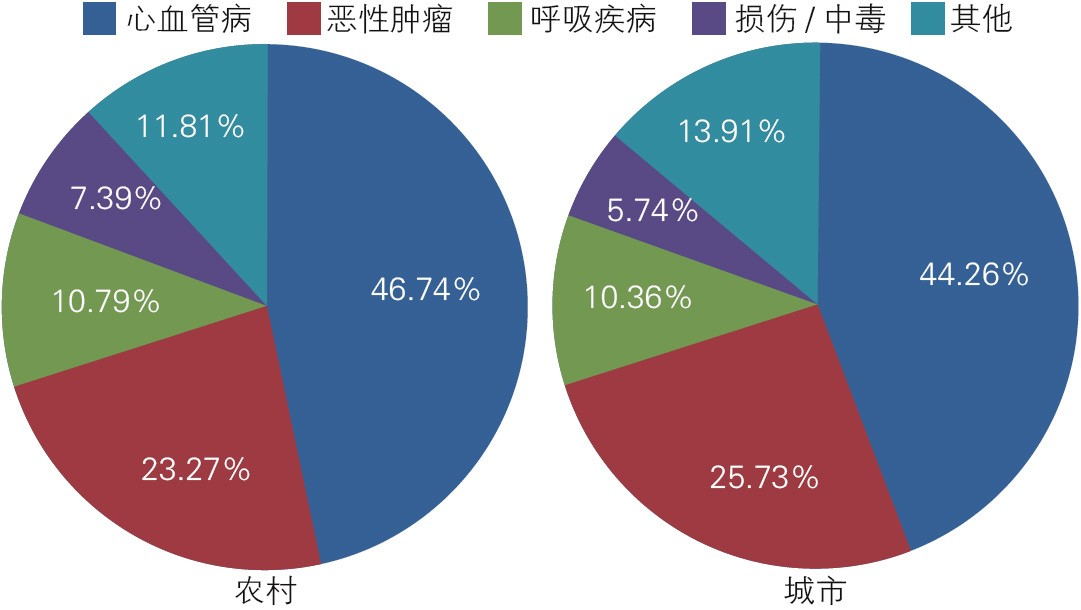
\includegraphics[width=.7\textwidth]{../assets/2019-death}
    \bicaption{2019年中国城乡居民主要疾病死因构成比\cite{Zhongguoxinxieguanjiankangyujibingbaogao20212022}}{Proportion of major causes of death among rural and urban in China in 2019}
    \label{fig:2019-death}
\end{figure}

不仅如此,根据世界卫生组织的统计\cite{CardiovascularDiseasesCVDs},心血管疾病也是全球的头号死因,每年死于心血管疾病的人数多于任何其它死因;2019年,估计有1790万人死于心血管疾病,占全球死亡总数的32\%。

同时,近年来新型冠状病毒(COVID-19)的爆发也加剧了心血管疾病的危害。证据显示,既往合并心血管疾病的患者更容易在新型冠状病毒感染后发展为重症患者,死亡风险更高,体征和症状更容易恶化\cite{zhangXinxingguanzhuangbingdufeiyanyuxinxieguanjibing2020}。

\subsection{心电监测的用途与原理}\label{subsec:monitoring}

尽早发现心血管疾病非常重要,这样就可以及时采取措施,减少疾病对患者健康的威胁\cite{CardiovascularDiseasesCVDs}。在各种心血管疾病的诊断方法中,心电图(Electrocardiogram,缩写为ECG)是最常用、最基本、最重要的一种,具有非侵入性、诊断快速、成本低廉、广泛可用等诸多优点\cite{Xinxieguanjibingzhenduanliuchengyuzhiliaocelue2007}。

心电图是对心电信号的记录。通过放置在皮肤上的电极可以检测到心脏的电活动,将电压与时间的关系绘制为二维图像就得到了心电图。

\subsection{常规心电图与动态心电图}\label{subsec:standard-holter}

心电图有两种主要类型:常规心电图(Standard ECG)和动态心电图(Holter ECG、Dynamic ECG或Ambulatory ECG)。

常规心电图,也被称为静息心电图(Resting ECG),是在患者保持静止状态时记录的心电图。常规心电图的记录需要在专业的医疗机构中进行,患者通常处于平躺状态,在四肢和胸部表面安装电极,电极检测心脏产生的电信号并将其传输到心电图仪器。常规心电图通常包含12个导联\footnote{这里的一个导联是指一对电极之间的电势差,比如II导联是指右臂电极和腿电极之间的电势差。另外,连接电极与心电图仪器的电缆也常被称为导联。本文中无特别说明的情况下,导联均指电势差而非电缆。},一次记录10秒,并打印在心电图纸上。如图~\ref{fig:ecg-paper-example} 所示是一张10秒12导联的常规心电图。

\begin{figure}[!ht]
    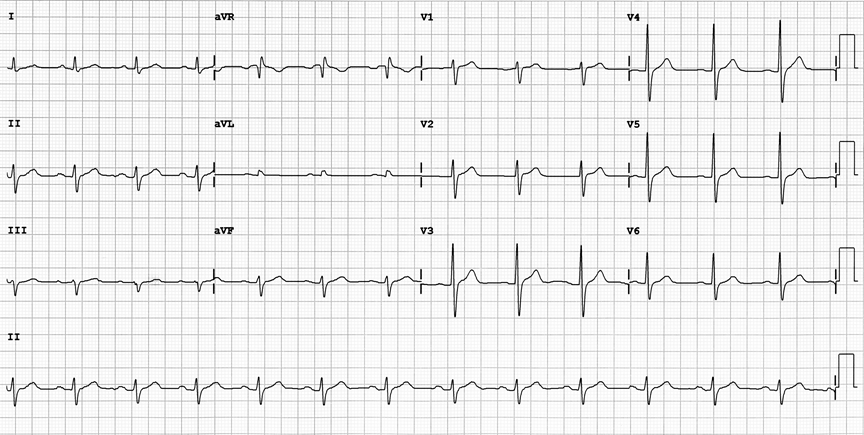
\includegraphics[width=\textwidth]{../assets/ecg-paper-example}
    \bicaption{一张10秒12导联的常规心电图}{A 10-second 12-lead standard ECG}
    \label{fig:ecg-paper-example}
\end{figure}

动态心电图则是在患者进行日常生活活动时记录的心电图。动态心电图的记录可以在几乎任何环境进行,只需要患者佩戴动态心电记录仪(Holter monitor)即可。动态心电记录仪是一种便携式可穿戴设备,可在较长时间内(24小时以上)记录心脏的电活动,有助于检出非持续性心律失常。统计显示,动态心电图在临床诊断中对心肌缺血及各种心律失常事件的检出率都明显高于常规心电图\cite{zhengDongtaixindiantuyuchangguixindiantuzhenduanguanxinbinghuanzhexinjiquexiejixinlushichangdelinchuangxiaoguobijiao2011}。

\subsection{\app 的意义}\label{subsec:app-significance}

动态心电图的数据量远远超过常规心电图,在显著提升了诊断精度的同时,也大幅提高了人工诊断的难度。人工进行大量数据的诊断识别,不仅使得医生过于疲劳、容易出错,也难以进行实时监测。于是,可以进行动态心电自动分析的\app 的需求就显而易见了。应用可以基于自动化的心电分析算法快速、准确地处理心电信号,为专业医疗人员节省时间,提高医疗服务的效率,降低医疗成本。使用\app 也更方便对患者进行实时监测,通过对心电数据进行实时分析可以及时发现患者的异常状况,为患者提供随时随地的医疗监护,降低心血管疾病对患者健康的威胁。


\section{相关技术与应用现状}\label{sec:status}

\subsection{动态心电自动分析技术现状}\label{subsec:automatic-analysis}

动态心电自动分析是指在采集到的动态心电信号的基础上,通过对其处理提取表征心脏状态的波形信息和特征参数,获取心脏工作状态的相关信息,然后利用这些特征信息分析、判别心电信号类型及所对应的疾病类型或健康水平,进而对心脏状态和健康状况进行预测\cite{jiXindianxinhaozidongfenxiguanjianjishuyanjiu2006}。

为了进行动态心电信号的自动分析,已经提出过许多相关算法。比如最著名的Pan-Tompkins算法\cite{panRealTimeQRSDetection1985}可以实时提取出心拍的位置,被广泛用于实时心率检测。U-Net模型\cite{ronnebergerUNetConvolutionalNetworks2015}作为一种生物医学图像分割模型也可以用于心拍提取,虽然无法实时给出结果,但在准确度等方面相较Pan-Tompkins等传统算法表现更好。基于ResNet\cite{heDeepResidualLearning2015}则可以训练心拍分类模型,用于自动识别每个心拍是否正常以及异常类型。

\subsection{国内外\app 现状}\label{subsec:app-status}

当前国内外已有不少\app ,其中一些使用了人工编写的传统心电分析算法\cite{zhengJiyukechuandaishebeideyidongjianhuAPP2019,wuYidongxindianjiancexitongdeyanjiuyushixian2018,chenYidongxindianxinxijianhuxitongjixindianjiancesuanfadeyanjiu2018,heJiyuyidongpingtaidexindianjianceyiliaoxitongdeshixian2017,gradlRealtimeECGMonitoring2012,wenRealtimeECGTelemonitoring2008},包括自适应双阈值法\cite{chenYidongxindianxinxijianhuxitongjixindianjiancesuanfadeyanjiu2018}、Pan-Tompkins算法\cite{gradlRealtimeECGMonitoring2012}以及一些原创的或基于已有算法改进的未命名的算法等;另一些\app 则使用了深度学习模型\cite{wangJiyushenduxuexideyidongyuanchengxindianjiancexitongshejiyushixian2020,singhSmartECGMonitoring2022,chenJiyushenduxuexidexindianfenximoxingdeshejiyuyouhua2021,liuJiyuyidongzhongduanfenxidekechuandairouxingxindianjiancexitong2021,wangEnablingSmartPersonalized2014,jinPredictingCardiovascularDisease2009}。

使用了深度学习模型的这些\app 按其整体架构可以大致分为两类:一类是在移动端只对数据进行简单统计处理,完整的算法模型则部署于服务端\cite{wangJiyushenduxuexideyidongyuanchengxindianjiancexitongshejiyushixian2020,singhSmartECGMonitoring2022},患者如果想获取完整的分析报告,则需要将数据上传至服务端后,等待服务端分析完成;这种应用架构的主要缺点是,患者能在移动端立即获取的结果较少,而完整分析结果可能因为网络质量差、服务端算力不足等原因而有较大延迟;另外,虽然患者不需要在自己的设备上运行相关算法,节省了一定开销,但上传与下载数据消耗的电量与流量成本不可忽视。另一类应用则采用了边缘计算架构,将深度学习模型部署在移动端,数据分析直接在移动端进行\cite{chenJiyushenduxuexidexindianfenximoxingdeshejiyuyouhua2021,liuJiyuyidongzhongduanfenxidekechuandairouxingxindianjiancexitong2021,wangEnablingSmartPersonalized2014,jinPredictingCardiovascularDisease2009},这样可以缩短延迟,节省带宽,并节省了高算力服务器的成本;然而,已有的少数此类应用都只实现了极简单的功能,旨在以演示应用验证模型正确性,并没有进行完整的应用开发,如图~\ref{fig:demos} 所示;此外,这些简单的演示应用均只进行了单一操作系统的开发。

\begin{figure}[!ht]
    \subcaptionbox{陈桂琛的应用\cite{chenJiyushenduxuexidexindianfenximoxingdeshejiyuyouhua2021}}{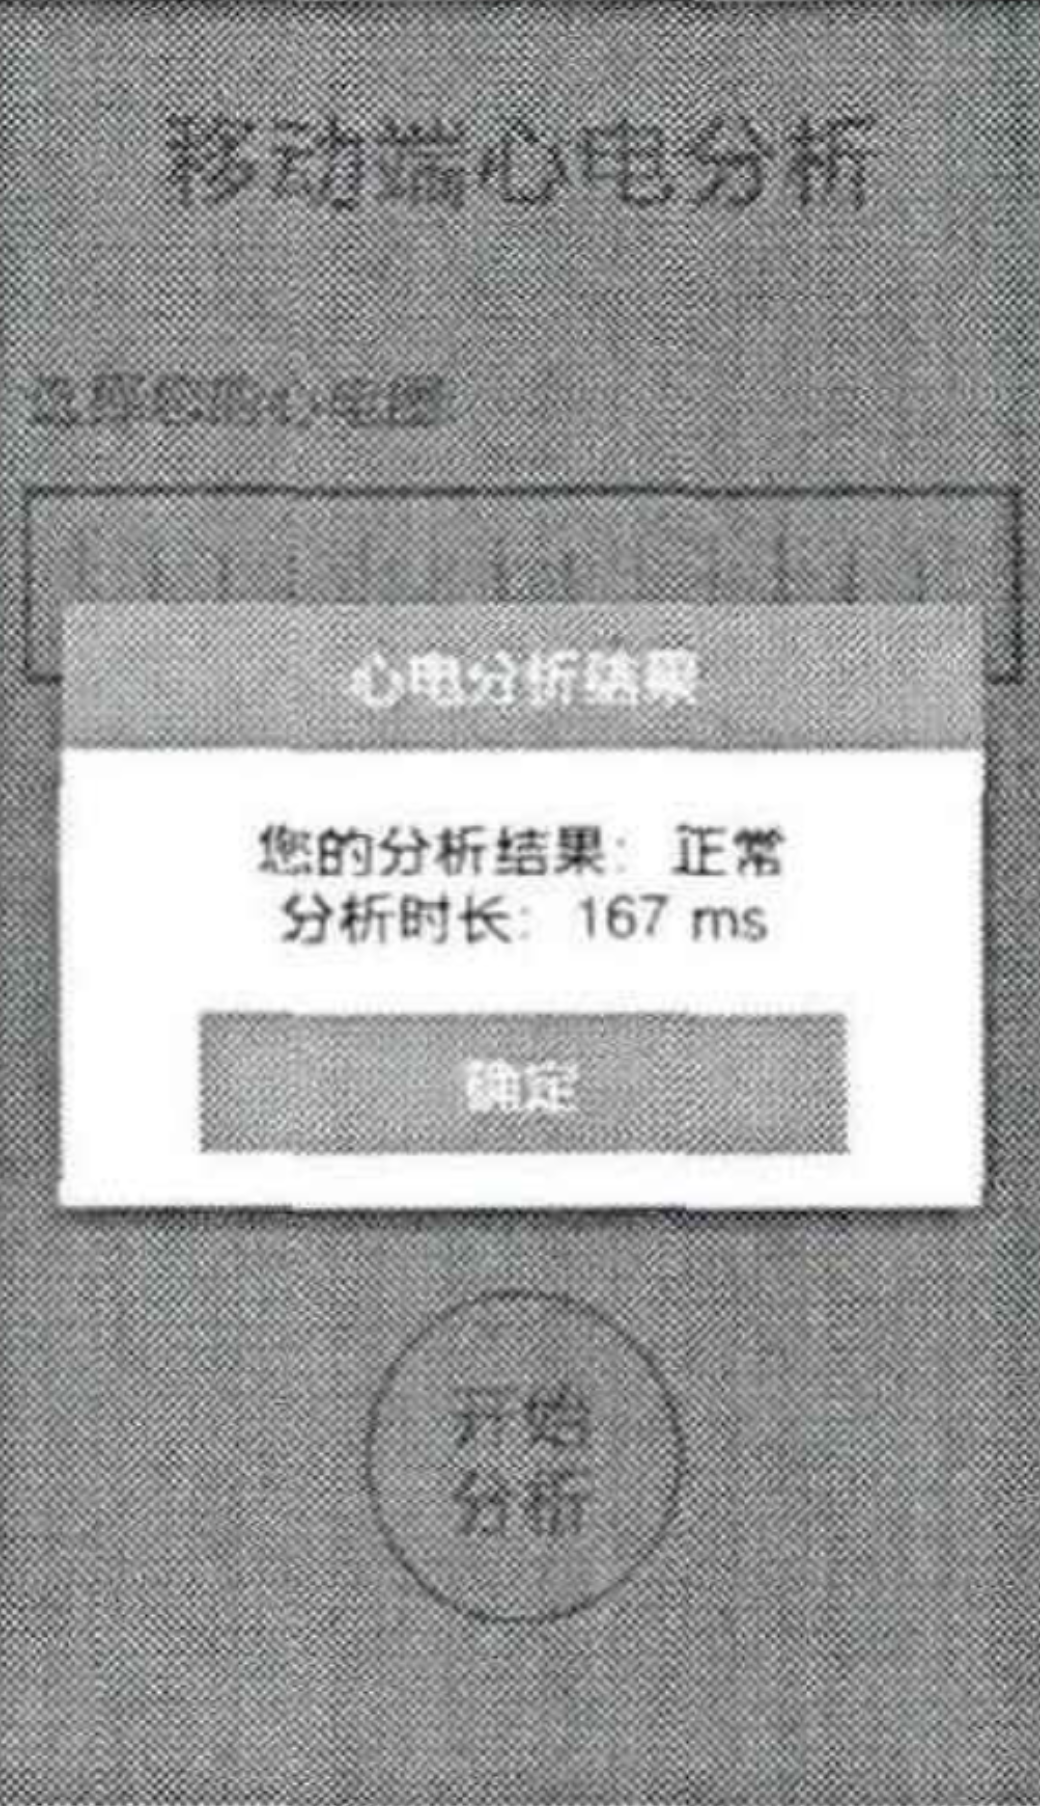
\includegraphics[height=9cm]{../assets/demo-0}}
    \subcaptionbox{刘荟的应用\cite{liuJiyuyidongzhongduanfenxidekechuandairouxingxindianjiancexitong2021}}{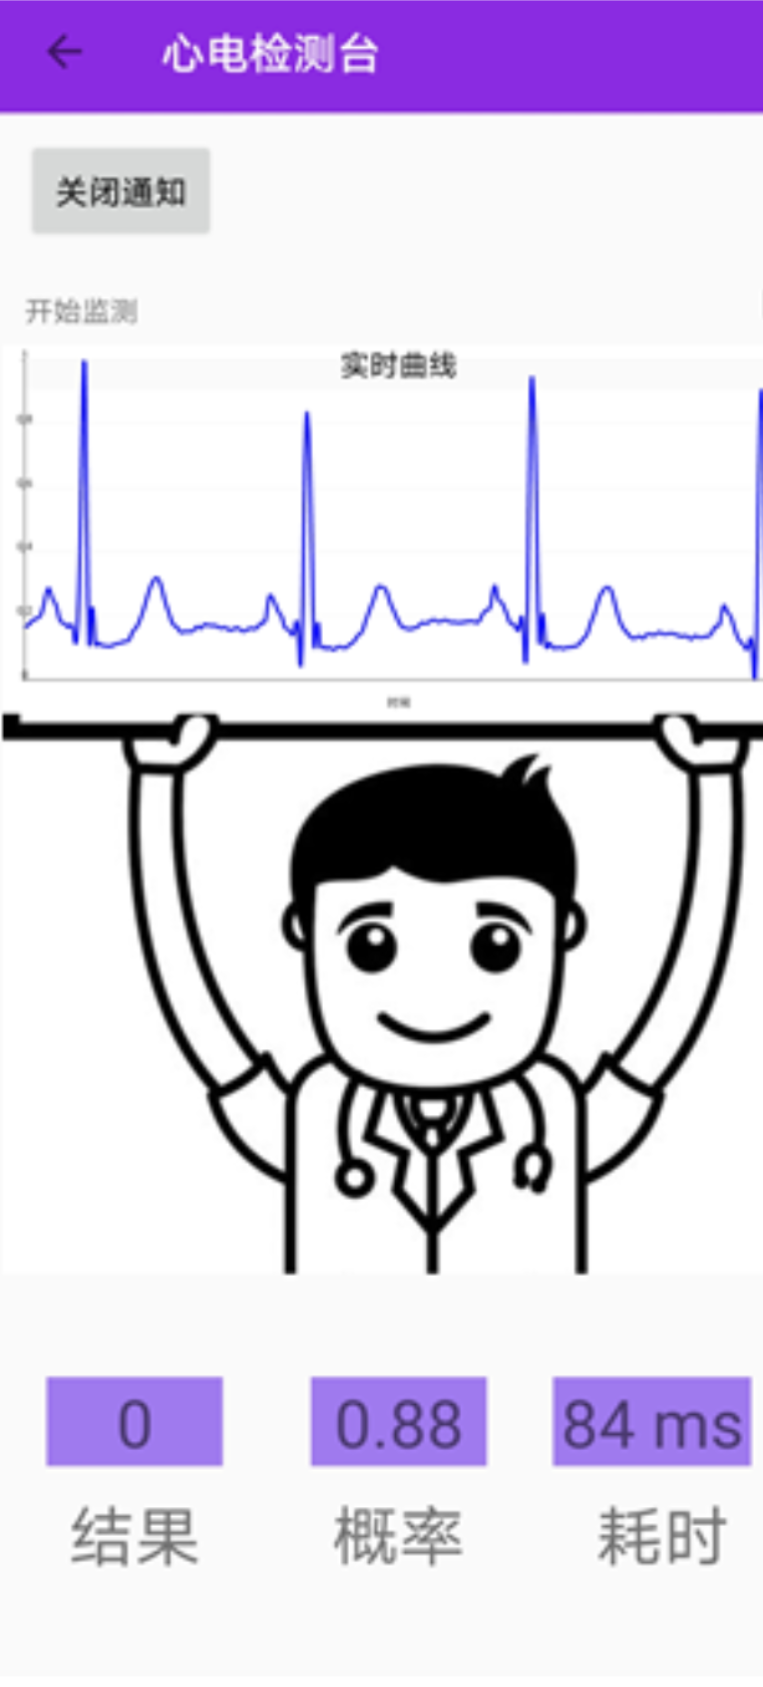
\includegraphics[height=9cm]{../assets/demo-1}}
    \subcaptionbox{Zhanpeng Jin等的HeartToGo\cite{jinPredictingCardiovascularDisease2009}}{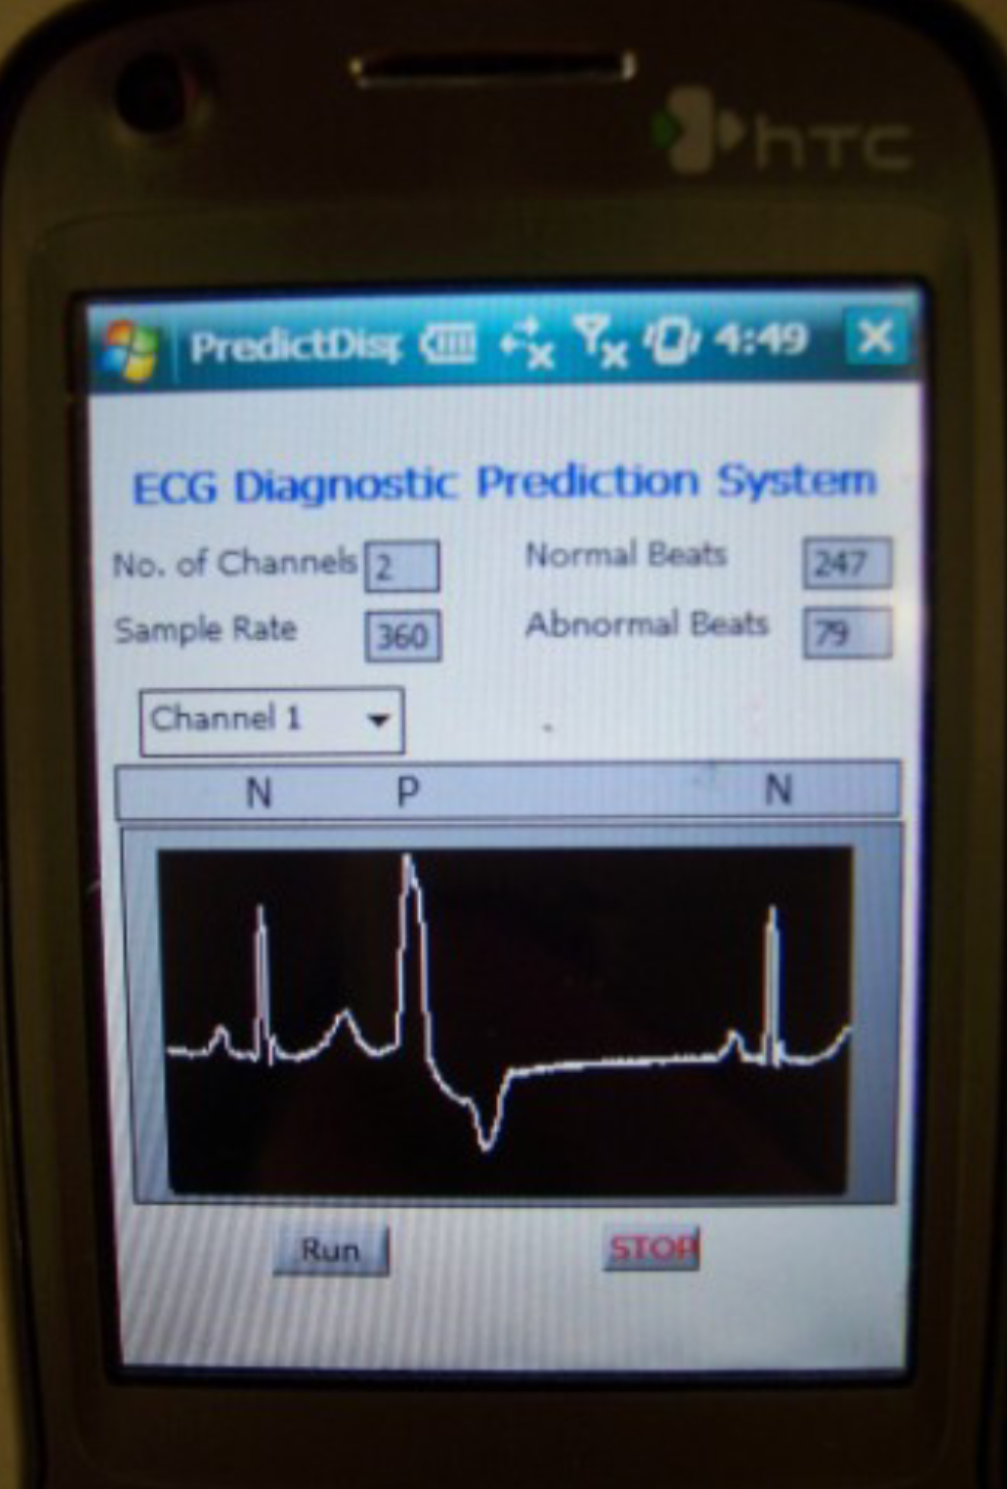
\includegraphics[height=9cm]{../assets/demo-2}}
    \bicaption{一些仅为验证模型而开发的简单演示应用}{Some demo apps only for model validation}
    \label{fig:demos}
\end{figure}


\section{本项目的主要工作}\label{sec:work}

本项目与~\ref{subsec:app-status} 节中所述的最后一类相似,也就是采用边缘计算架构,将深度学习模型部署在移动端,数据分析直接在移动端进行。本项目与上文提及的已有的同类应用的主要差别在于其选题来源于导师的心电图课题的子项目,是在已经基于PyTorch完成了相关算法模型\cite{songDongtaixindiantudezhinengjiancesuanfayanjiuyuyingyong2022}的情况下进行的,在项目之初就已有较好的人工智能算法模型的技术支撑。于是,相比于偏重算法研究而在实际的应用开发方面较为欠缺的其他项目,本项目的主要工作在于将已有的算法模型与移动应用开发技术进行整合,以实现一个较为完整的\app ,目标是最终投入到实际的生产环境中供患者使用。

在项目过程中,首先对应用的需求进行了分析,明确了应用的功能性需求和非功能性需求。然后为了满足需求进行了技术选型,明确了项目要使用的技术栈。之后对应用的整体架构和各个模块进行了设计。在开发阶段,完成了已有算法的移植与优化,以及应用程序本身的开发。最后,对应用进行了测试,以确保其可以满足需求。


\section{论文组织结构}\label{sec:structure}

本文分为7个章节,各章节的主要内容如下:

\begin{description}
    \item [1、绪论] 介绍了本项目的背景与意义、相关技术与应用现状、本项目的主要工作、本文的组织结构。
    \item [2、相关技术介绍] 对本项目使用的相关技术进行了介绍,包括Flutter相关的移动应用开发技术和算法相关的一些技术。
    \item [3、可穿戴动态心电监测应用的需求分析] 对应用进行了需求分析,明确了应用的目标用户、功能性需求、非功能性需求、项目可行性。
    \item [4、可穿戴动态心电监测应用的设计] 对应用的整体架构和各个模块以及数据库进行了设计。
    \item [5、可穿戴动态心电监测应用的开发] 介绍了应用的开发过程,包括开发环境与工具、算法的实现与移植、应用程序各个模块的实现等。
    \item [6、可穿戴动态心电监测应用的测试] 包含项目的测试环境、测试数据、测试方法、测试用例等。
    \item [7、总结与展望] 总结了本项目的主要工作,对未来的工作进行了展望。
\end{description}

    %! suppress = UnresolvedReference


\chapter{相关技术介绍}\label{ch:tech}


\section{Flutter跨平台应用程序开发框架}\label{sec:flutter}

\subsection{使用跨平台应用程序开发框架的意义}\label{subsec:why-framework}

要开发一个面向移动终端的\app ,首先要考虑的是该应用支持哪些移动平台。根据2023年3月的数据\cite{MobileOperatingSystem},在中国的移动平台操作系统占有率中,Android系统以76.15\%名列第一,iOS系统以23.28\%位居第二,这两个最主流的移动平台操作系统占据了绝大部分市场份额。因此,本应用开发的目标平台选定为Android和iOS。

Android和iOS开发的各种技术可以分为两大方向:原生应用程序开发和跨平台应用程序开发。构建传统的原生应用程序需要维护两个不同的代码库,分别为Android和iOS平台编写代码,通常意味着需要分别使用Kotlin/Java和Swift/Objective-C来编写两份高度相似的代码。而跨平台应用程序开发框架则可以通过一套代码库同时为Android和iOS平台构建应用程序,降低了开发人员的学习成本,缩减了开发时间,提高了开发效率。

\subsection{Flutter简介}\label{subsec:flutter}

Flutter是一个由Google开源的跨平台应用程序开发框架,仅通过一套代码库就能构建精美的、原生平台编译的跨平台应用\cite{FlutterBuildApps}。

Flutter对Android和iOS平台均有良好支持,此外还支持Windows、Linux、macOS、Web等平台\cite{SupportedDeploymentPlatforms}。基于Flutter框架进行开发不仅可以避免为Android和iOS平台分别编写大量相似的代码,还可以方便未来将部分不依赖于移动端特性的功能(比如历史心电展示等)的相关代码在其他平台(比如Web端)复用。

\subsection{Flutter与其他框架的对比}\label{subsec:flutter-compare}

Flutter并不是唯一一个支持Android和iOS平台的跨平台应用程序开发框架。在本项目的选型过程中也考虑了其他几个经常被与Flutter进行比较的同类框架,包括React Native\cite{ReactNativeLearn}、Xamarin\cite{XamarinOpensourceMobile}、Ionic Creator\cite{IonicFrameworkCrossPlatform}。

关于这几个框架,最先被对比的是其热度。以近一年的Google趋势作为标准,对比结果如图~\ref{fig:google-trends} 所示。

\begin{figure}[h]
    \centering
    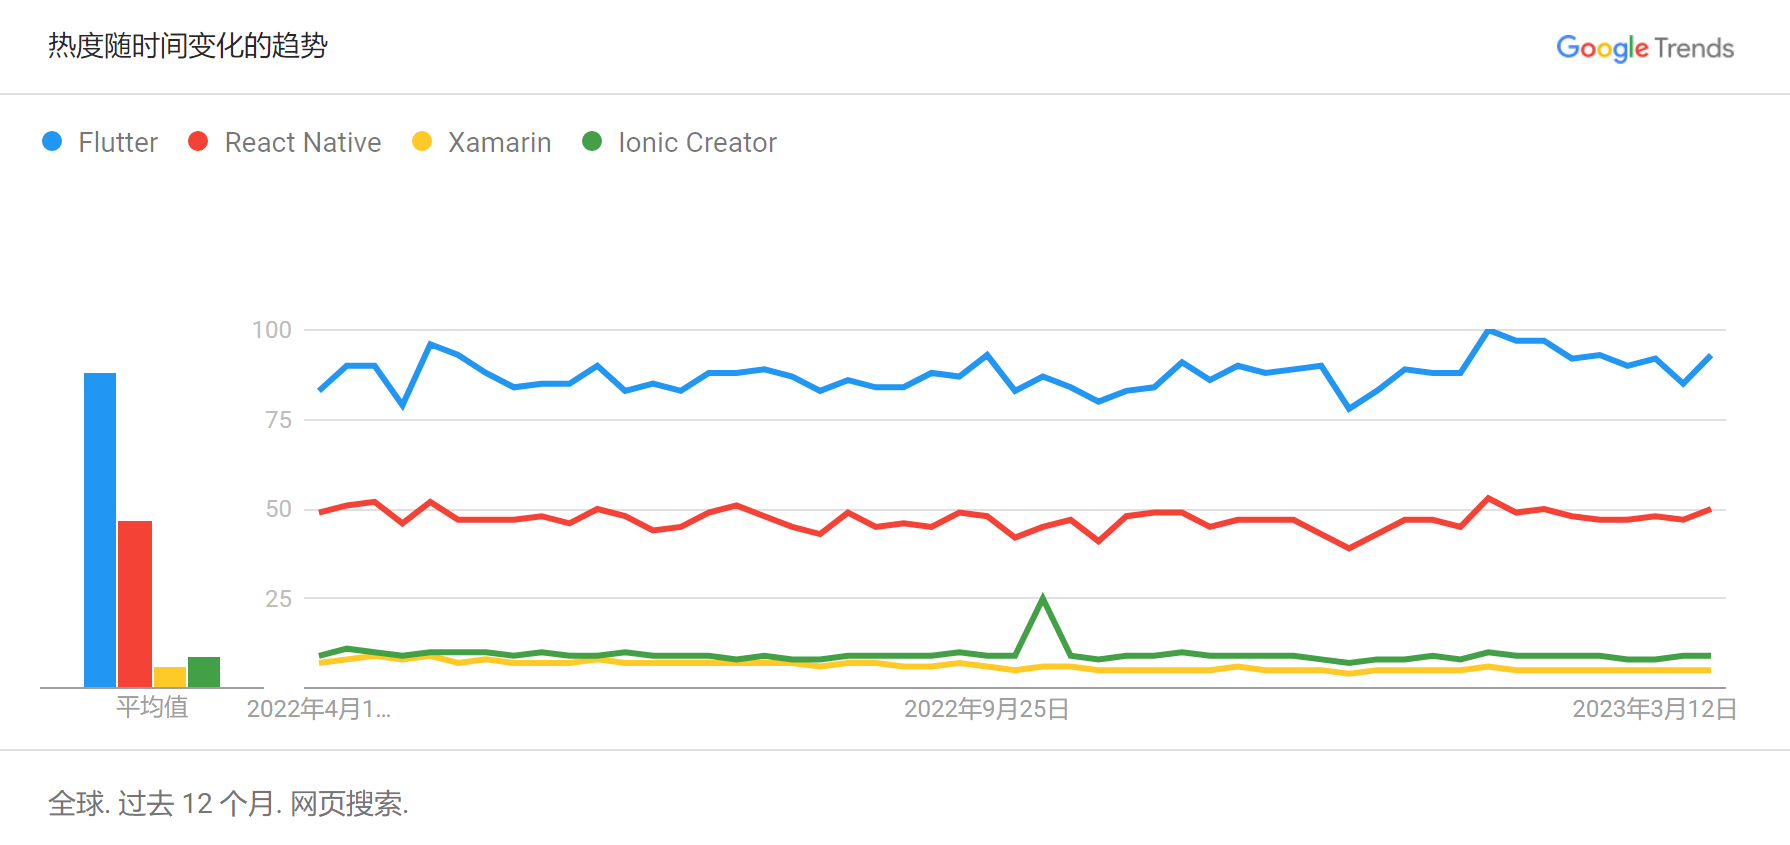
\includegraphics[width=\textwidth]{../assets/google-trends}
    \bicaption{Flutter与其他框架的Google趋势}{Google Trends for Flutter and other frameworks}
    \label{fig:google-trends}
\end{figure}

从图中可以看出,Flutter和React Native的热度远远高于Xamarin和Ionic Creator。热度高意味着其社区更加活跃,生态更为优秀,更容易找到相关的资料和技术支持,也更容易利用社区已经开发过的包,这些对于项目开发来说都是非常重要的。因此,Xamarin和Ionic Creator在本项目的选型过程中最先被排除。

之后需要对比的是Flutter和React Native。从热度上来看,两者的热度都比较平稳,Flutter长期保持在React Native的两倍左右,这意味着Flutter应当被优先考虑,但还不足以作为决定性理由。因此,需要进一步对比这两个框架的特性。

React Native是由Meta(前身为Facebook)于2015年开源的跨平台应用程序开发框架。正如其名称所暗示的,React Native和React(一个流行的Web框架)的关系十分密切,这既是优点也是缺点。从优点的方面来说,React Native非常适合已有React开发经验但没有移动平台开发经验的开发者快速上手,也适合将已有的基于React的Web项目迁移至移动端,但这两点对于本项目来说都没有明显意义。另一方面,由于和React的紧密联系,基于React Native的应用需要使用JavaScript和CSS编写,代码会在JavaScript引擎下解释执行,并通过序列化消息与本机代码桥接通信以渲染原生组件。JavaScript本来就不是一种以性能见长的语言,额外的桥接翻译层更使得其性能较之原生应用程序相去甚远。

作为对比,Flutter是Google于两年后(2017年)开源的,其设计上明显借鉴了React Native,与其一样使用响应式风格的界面编写方式。主要差别在于Flutter是编译成原生代码运行,直接接管并控制屏幕上的每一个像素,由此可以避免使用JavaScript桥接导致的性能问题。

除了上述的性能优势之外,Flutter还在热重载、IDE集成、内置调试工具等方面相较其他框架更为优秀。最终,基于以上所有考虑,本项目选择了Flutter作为开发框架。

\subsection{Dart语言}\label{subsec:dart}

Dart是由Google开源的编程语言,专门针对用户界面(User interface,缩写为UI)的创造进行优化,可编译为移动平台、桌面平台的二进制文件和Web平台的Javascript代码\cite{DartProgrammingLanguage}。Dart最初于2011年发布,原本是打算捆绑于Chrome浏览器来替代JavaScript,但后来由于各种因素而未能成功。在Flutter开发团队选择了Dart作为开发语言之后,两者的关系便愈加紧密,Dart也因此得到了更多的关注,并顺应Flutter框架的需求进行了许多更新迭代。时至今日,Dart与Flutter可以说是处于完全捆绑的状态,基于Flutter框架进行开发几乎是学习并使用Dart语言的唯一目的,使用Dart语言也是基于Flutter框架进行开发的必要条件。

Dart是一种多范式的语言,支持函数式、命令式、面向对象、反射式的写法,语法风格近似于C++与Java的混合,支持抽象类、泛型、类型推断、自动内存管理、空安全等其他语言中较为常见的特性,也有Mixin、Extension方法等其他语言中不太常见的特性。因篇幅限制,本文不便对Dart的诸多特性进行完整介绍,这里仅对后文必须涉及,且与其他语言有明显差异的部分特性进行简单说明。

\subsubsection{外部函数接口}\label{subsubsec:ffi}

外部函数接口(Foreign function interface,缩写为FFI)是一种机制,指用一种编程语言编写的程序可以调用另一种编程语言编写的功能。比如在C++中可以指定 \lstinline[language=C]{extern "C"} 来要求编译器在调用约定、名字重整等方面遵循C语言的标准\footnote{这一特性在C++中被称为语言链接(Language linkage)。},从而实现与C语言之间的双向FFI。

Dart作为一种专精于UI开发的语言,在其他方面的生态较为薄弱。作为一种弥补方式,Dart实现了与许多其他语言之间的FFI,比如在Web上可以与JavaScript互相调用,在macOS和iOS上可以与Swift或Objective-C互相调用,在Android、Windows、macOS、Linux上可以与Kotlin或Java互相调用,以及对本项目来说最重要的——在除Web以外的所有平台可以与C语言直接进行交互,而无须像React Native等框架那样通过Java等中间层进行间接调用,这使得Dart与C语言之间的FFI十分高效。由于C++代码也可以通过指定 \lstinline[language=C]{extern "C"} 来编译为与C语言格式相同的接口,这意味着本应用的部分功能可以直接使用C++编写,从而充分利用C++的性能、生态、跨平台性等优势。

在项目的开发过程中,使用C++编写了两部分代码供Dart FFI调用,分别是Pan-Tompkins算法和基于LibTorch的人工智能算法,在后文会详细介绍。

\subsubsection{Isolate}\label{subsubsec:isolate}

Isolate\footnote{该术语没有常用的中文译名,故本文中直接使用英文原名。}是Dart中的一种介于线程与进程之间的概念。在Dart程序中,所有的代码都在isolate中运行。每一个isolate都有独立的运行线程和独立的堆内存,从而确保isolate之间互相隔离,无法互相访问状态。相比于常规的线程,这样的实现并不会共享内存,所以也不需要担心互斥锁和其他锁等问题。相对地,由于无法与其他isolate共享可变对象,isolate之间的通信必须使用消息机制。

Dart程序有一个默认的主isolate,在Flutter应用中也称为UI isolate,因为UI的更新都是在主isolate中进行的。在本应用中,数据库查询等可能较为耗时的操作都是放在其他isolate中异步执行的,以避免阻塞UI isolate导致UI卡顿。

\subsection{项目使用的Flutter包}\label{subsec:flutter-packages}

尽管Flutter SDK本身已经包含了大量的基础组件,但是在实际开发中,还是经常需要额外使用官方或社区开发的Flutter包来实现一些特定的功能。本项目所使用的Flutter包总计有上百个,其中一些包的使用比较简单,比如URL Launcher包只是用来在各个平台提供在浏览器中打开指定的URL的功能;而另一些包则在项目开发的各个阶段有着广泛的影响,比如Isar包的特性直接影响了本项目数据库的设计、实现与测试。

由于项目使用的Flutter包非常多,而且作用分散在项目的各个阶段、各个模块,在此处一一介绍会使得本节过于冗长且难以理解,本文在后续章节涉及到相关Flutter包时再对各个包分别进行说明。另外,所有包的相关文档均可在\url{https://pub.dev/}上找到,由于数目众多,本文不在参考文献中分别列出。


\section{项目使用的Python包与C++中的对应替代}\label{sec:python-cpp-packages}

\subsection{将Python代码迁移至C++的原因}\label{subsec:why-cpp}

本项目使用的用于心电信号分析的人工智能算法最初是使用Python编写的。为了在面向移动终端的应用中使用这些算法,考虑了各种可能的技术方案。

\subsubsection{移动端直接执行Python代码的方案}\label{subsubsec:run-python}

最简单的一个方案是设法在移动端直接执行Python代码。这种方式在移动应用开发中很少被使用,主要是基于时间上和空间上这两个方面的顾虑。从时间上来说,Python语言的执行效率较低,在设备性能相对较差的移动端表现得更为明显;不过本应用中人工智能算法的执行时间占比并不大,仅仅是每10分钟调用一次,一次执行数秒而已,所以这一缺点也并非不可接受。从空间上来说,将Python语言的运行环境打包进应用会导致应用的安装包体积更大;但此算法所需要的Torch模型文件本身就已有60多MB,相较之下Python的运行环境所额外占据的大小并不是很明显。因此,常见的关于性能或安装包大小的顾虑并不能构成否定本方案的充分依据。之后考虑了在移动端执行Python代码的各种方式。

PyQtDeploy\cite{RiverbankComputingIntroduction}、QPython\cite{QPythonPythonAndroid}、Termux\cite{Termux}等工具可以用于在移动端执行Python代码,但未提供可供Java、Dart等语言调用的接口,因此无法在本项目中使用。

Kivy\cite{KivyCrossplatformPython}提供了Python与Java、Objective-C的交互,但是缺少对于PyTorch的支持,而这一依赖难以替代,所以Kivy也无法在本项目中使用。

Chaquopy\cite{EasiestWayUse}提供了PyTorch的支持。尽管最高只支持1.8.1版本,但算法原本所依赖的版本甚至比这更旧,所以PyTorch的使用没有问题。但是,Chaquopy仅支持Android平台,而不支持iOS平台,所以无法完全满足本项目的需求。

BeeWare\cite{WriteOnceDeploy}在Chaquopy之上增加了对iOS平台的支持,但是需要将整个应用都使用Python编写,这样就无法通过仅在少数部分调用Python来避开本小节最初提到的性能问题,因此也不是可行的方案。

综合以上调查结果,可以认定移动端直接执行Python代码的方案并不可行。因此,必须将原本使用Python编写的算法迁移至其他语言。

\subsubsection{使用Dart实现相关算法的方案}\label{subsubsec:python-dart}

\todo{}

\subsubsection{使用C++实现相关算法的方案}\label{subsubsec:python-cpp}

\todo{为什么需要C++中的对应替代?(需要将Python算法迁移至C++,部分关键依赖无法消除。)}

本项目的一部分工作是将已有的使用Python编写的算法迁移至C++。

\subsection{PyTorch与LibTorch}\label{subsec:pytorch-libtorch}

\todo{什么是PyTorch?}

\todo{什么是LibTorch?}

\todo{为什么选择LibTorch而不是PyTorch Mobile、MNN、NCNN等?(PyTorch官方支持,接口设计高度相似,引用官方文档中相关说明。)}

\subsection{NumPy与NumCpp}\label{subsec:numpy-numcpp}

\todo{什么是NumPy?}

\todo{什么是NumCpp?}

\todo{为什么选择NumCpp而不是Eigen等?(接口与NumPy更相似。)}

\subsection{pytest与Catch2}\label{subsec:pytest-catch2}

\todo{什么是pytest?(关于名字:pytest的官方名称即为全小写形式,即使在位于句首的情况下也是如此。)}

\todo{什么是Catch2?}

\todo{为什么选择Catch2而不是Google Test、Boost Test等?(更简单,本项目的C++部分没有编写复杂的测试用例的需求。)}

\subsection{nlohmann::json}\label{subsec:nlohmann-json}

\todo{为什么需要nlohmann::json?(Python标准库有JSON支持,C++没有,需要第三方库。)}

\todo{什么是nlohmann::json,不是其他JSON库?(接口简单。虽然性能有劣势,但只是用于读取少量测试数据,速度不重要。)}

    %! suppress = UnresolvedReference


\chapter{\app 的需求分析}\label{ch:req}


\section{应用面向的用户群体}\label{sec:target-user}

本应用的目标用户是佩戴可穿戴动态心电信号监测设备的院外患者。由于心血管疾病的发病率随着年龄增长而增加\cite{Zhongguoxinxieguanjiankangyujibingbaogao20212022},有动态心电监测需求的患者也以中老年人为主。除了常规的功能性需求分析之外,本项目也结合用户群体的特征进行了额外的非功能性需求分析以及相关的设计和实现。


\section{应用的功能性需求分析}\label{sec:func-req}

\todo{应用有哪些功能性需求?(参考开题报告,结合之后实际开发的情况做些调整。)}


\section{应用的非功能性需求分析}\label{sec:nonfunc-req}

\subsection{易用性}\label{subsec:usability}

因为大部分中老年的用户没有丰富的移动设备使用经验,所以设计一个简单直观、易于使用的应用程序很重要。界面设计应避免使用复杂的元素,以尽量简洁清晰为目标。

此外,由于一般患者通常不会具备专业的医学知识,所以应用程序内应该尽可能地避免使用过于晦涩难懂的专业术语。同时,对于应用内无法避免使用的部分术语应该提供明显且易于理解的解释,以便用户理解其含义。

\todo{还有哪些非功能性需求?(至少把开题报告里面那些抄过来。)}

\section{项目的可行性分析}\label{sec:feasibility}

\todo{项目是否可行?为什么?(事实证明是可行的,但还是得站在项目开始前的视角分析一下。)}

    %! suppress = UnresolvedReference


\chapter{\app 的设计}\label{ch:design}


\section{应用的整体架构设计}\label{sec:arch-design}

本应用的整体架构如图~\ref{fig:model} 所示。因空间有限,此处对部分模块进行了合并与省略,后续小节会展开介绍。

\begin{figure}[!ht]
    \centering
    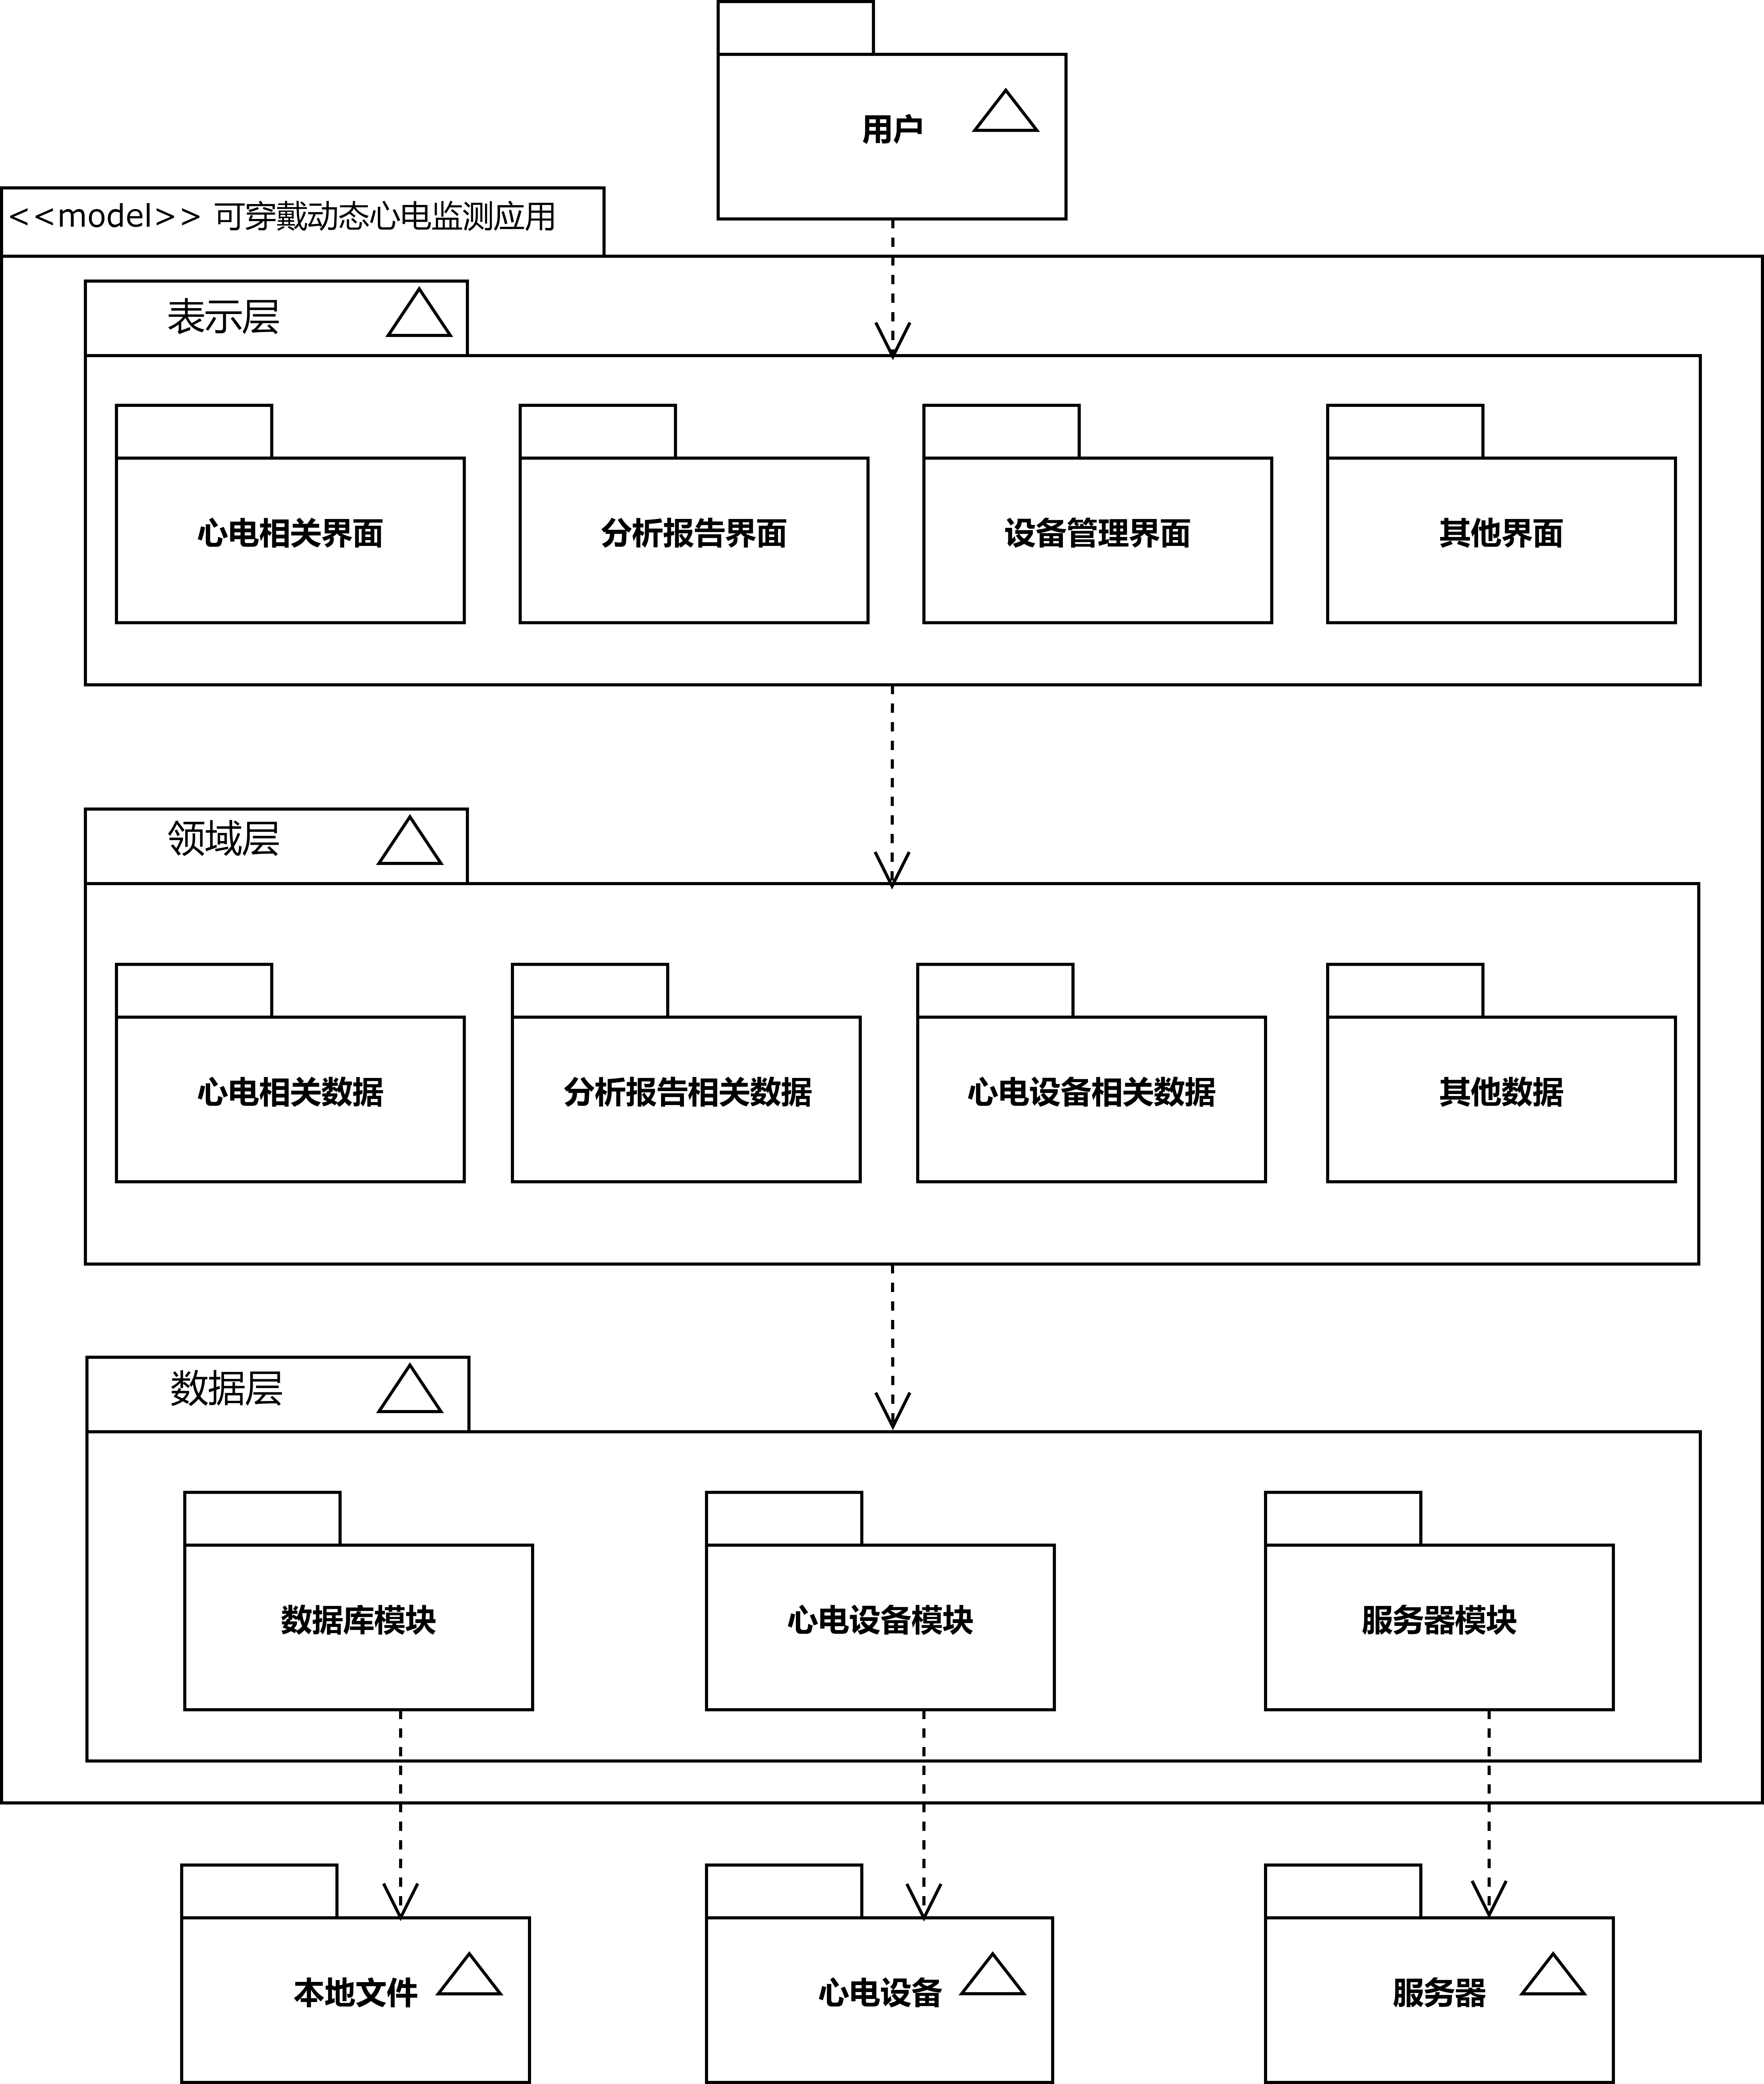
\includegraphics[width=.9\textwidth]{../assets/model.drawio}
    \bicaption{应用的整体架构}{Architecture of the app}
    \label{fig:model}
\end{figure}

本应用使用了Riverpod架构模式\cite{bizzottoFlutterAppArchitecture},其与MVC等传统模式有较大差别,且由于提出较晚而知名度不高,因此本节顺带对该模式进行简单介绍。

在设计应用程序时选择正确的应用架构至关重要,过于简陋的设计会使得代码整体缺乏组织性,过于繁复的设计则会阻碍代码的修改迭代。自最经典的MVC架构以来,已有许多流行的应用架构被相继提出。其中一些对原始的MVC架构进行改动后仍沿用其名称,导致MVC这一术语的含义愈加模糊;另一些变体则被命名为MVP、MVVM、MVC+S等MV*,或是如Clean Architecture等另起炉灶。这些经典的架构模式很难原样照搬至Flutter框架,即使强行在Flutter中进行实现也只会使得代码结构不伦不类。在探索Flutter适用的应用架构的过程中,社区已经提出了许多新模式,如BLoC、Stacked等。而在本应用的架构设计中,采用的则是Andrea于2022年初提出的Riverpod架构模式。

Flutter曾经有一个流行的状态管理包Provider,该包也是上述的BLoC、Stacked等架构模式的基础。后来,由于Provider包的设计逐渐暴露出一些难以解决的问题,其开发者将该包进行了大幅重写,并因其与旧版本不兼容而改名为Riverpod(对Provider中字母的重组)重新发布,Andrea提出的该架构模式因基于Riverpod包而命名为Riverpod架构模式。

该架构模式由三层或四层组成,从上至下分别是表示(Presentation)层、可选的应用(Application)层、领域(Domain)层、数据(Data)层。

\subsection{表示层}\label{subsec:presentation-layer}

表示层类似于MVC中的View和Controller,或是MVVM中的View和ViewModel,以及Android应用架构指南\footnote{\url{https://developer.android.com/jetpack/guide\#recommended-app-arch}}中的UI层。该层包含用户可见的UI组件以及相关的特定于某个组件的状态与交互逻辑。由于Flutter采用了响应式的设计思想,UI本身与其对应的状态的关系极为密切,因此在Riverpod架构中,将MV*中的Model以外的两层进行了合并。在本应用中,该层包含实时心电界面、历史心电界面、分析报告界面等内容。

\subsection{应用层}\label{subsec:app-layer}

应用层类似Android应用架构指南中的领域层(两边对领域层这一术语的使用不一致),并且与其一样是可选的。这是因为并非所有应用都具有复杂的业务逻辑,也并非所有业务逻辑都需要被提取出来以便重用。在Riverpod架构中,如果不需要应用层,则可以直接省略这一层。在本应用中,由于应用的业务逻辑较为简单,因此并未使用该层。

\subsection{领域层}\label{subsec:domain-layer}

领域层类似于MV*中的Model。该层包含领域模型,即应用程序中的数据及其相关的方法。由于领域层在各种架构模式中被广泛使用(尽管命名可能不同),此处不作详细介绍。在本应用中,该层包括心电数据、心拍数据、应用设置数据等模型。

\subsection{数据层}\label{subsec:data-layer}

数据层类似Android应用架构指南中的数据层。该层包含与外部数据源通信的相关代码,负责将领域模型与底层的数据源的实现细节进行隔离,将从数据源获取的原始格式的数据(如JSON等)转换为领域层中的领域对象(应用中自定义的数据类),有时也执行数据缓存等操作。在本应用中,该层包含与数据库、心电监测设备、服务器进行通信的相关代码。


\section{应用各个模块的设计}\label{sec:app-design}

\subsection{心电模块的设计}\label{subsec:ecg-design}

心电模块的整体架构如图~\ref{fig:model-ecg} 所示。因Riverpod架构模式未指明外部函数接口和后台定时任务属于哪一层,本图将其绘制于已有层次之外。

\begin{figure}[!ht]
    \centering
    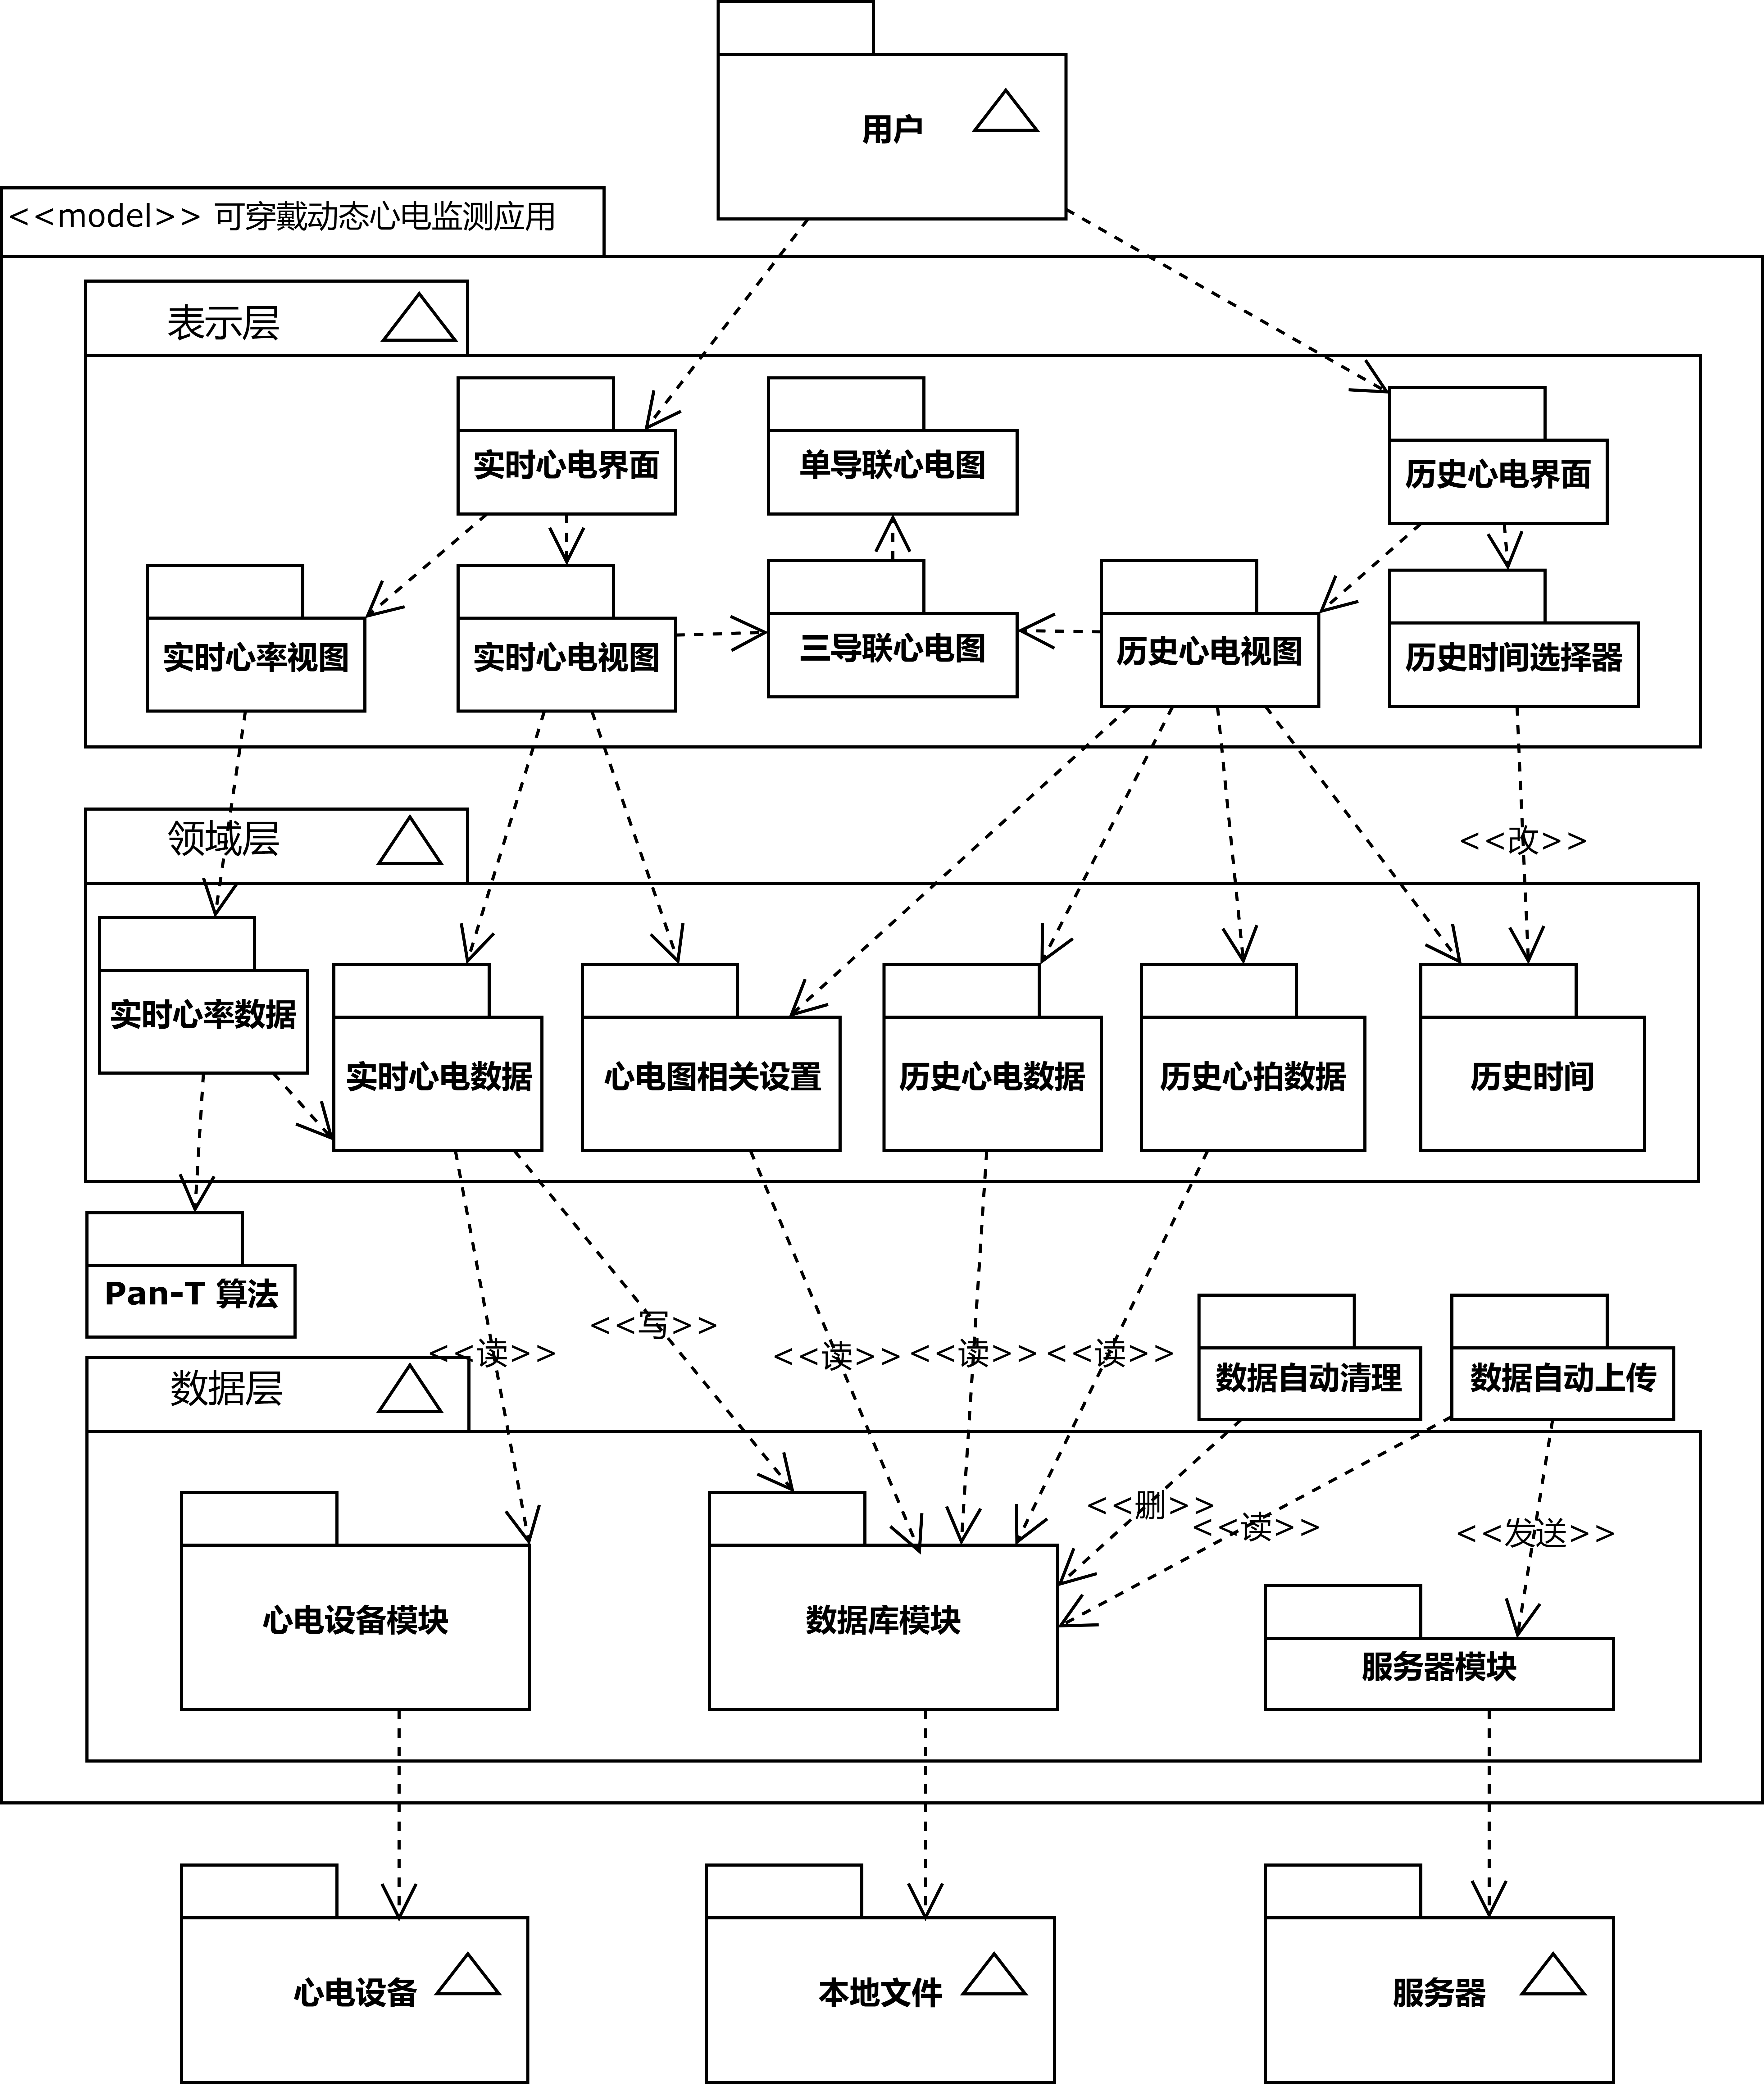
\includegraphics[width=.8\textwidth]{../assets/model-ecg.drawio}
    \bicaption{心电模块的架构}{Architecture of the ECG module}
    \label{fig:model-ecg}
\end{figure}

心电模块可以大致划分为实时心电模块和历史心电模块这两个子模块,不过两者在各个层级的重合部分较多,在最终的实现中也有不少共享的代码,因此一并归于心电模块。

\subsubsection{表示层}

心电模块的表示层中为用户提供了两个心电相关的界面,分别是实时心电界面和历史心电界面。实时心电界面包含实时心电视图和实时心率视图,历史心电界面则包含历史心电视图和历史时间选择器。实时心电视图与历史心电视图均为心电图的显示,因此提取其共享部分作为三导联心电图UI组件。然后,由于三个导联的心电图之间也高度相似,在三导联心电图之中再提取出单导联心电图UI组件,以免编写重复代码。

\subsubsection{领域层}

心电模块的领域层中,实时心率数据由实时心率视图读取;实时心电数据由实时心电视图读取,也被用于心率数据的获取,并被存入数据库;心电图相关设置数据由实时心电视图和历史心电视图读取(实际上有不同的设置项,但在该设计层次无须细分);历史心电数据和历史心拍数据由历史心电视图读取;历史时间由历史时间选择器进行修改,由历史心电视图读取,并被用于对历史心电数据和历史心拍数据的查询。

\subsubsection{其他层}

Pan-Tompkins算法(图中简写为Pan-T算法)模块以C++语言实现,通过Dart FFI被调用,用于通过实时心电数据得到心拍位置,进而得到心率数据;另外,Pan-Tompkins算法所给出的心拍位置也会作为未知类型的心拍存入数据库,以供历史时间选择器使用(跳转至上一个或下一个心拍的时间),为了保证图像清晰而并未在图中标出。数据自动清理模块和数据自动上传模块都是后台定时运行的自动任务,对用户而言并不可见;数据自动清理模块负责清理较旧的数据,避免应用占用空间过多;数据自动上传模块负责将数据库中的数据上传至服务器作为备份。

\subsubsection{数据层}

心电模块需要用到数据层中的所有三个子模块。心电设备模块用于提供实时心电数据;数据库模块用于实时心电数据的写入、心电相关设置与历史心电数据的读取、来源于Pan-Tompkins算法的心拍位置的写入、历史心拍数据的读取;服务器模块用于数据上传。

\subsection{分析报告模块的设计}\label{subsec:analytics-design}

分析报告模块的整体架构如图~\ref{fig:model-analytics} 所示。

\begin{figure}[!ht]
    \centering
    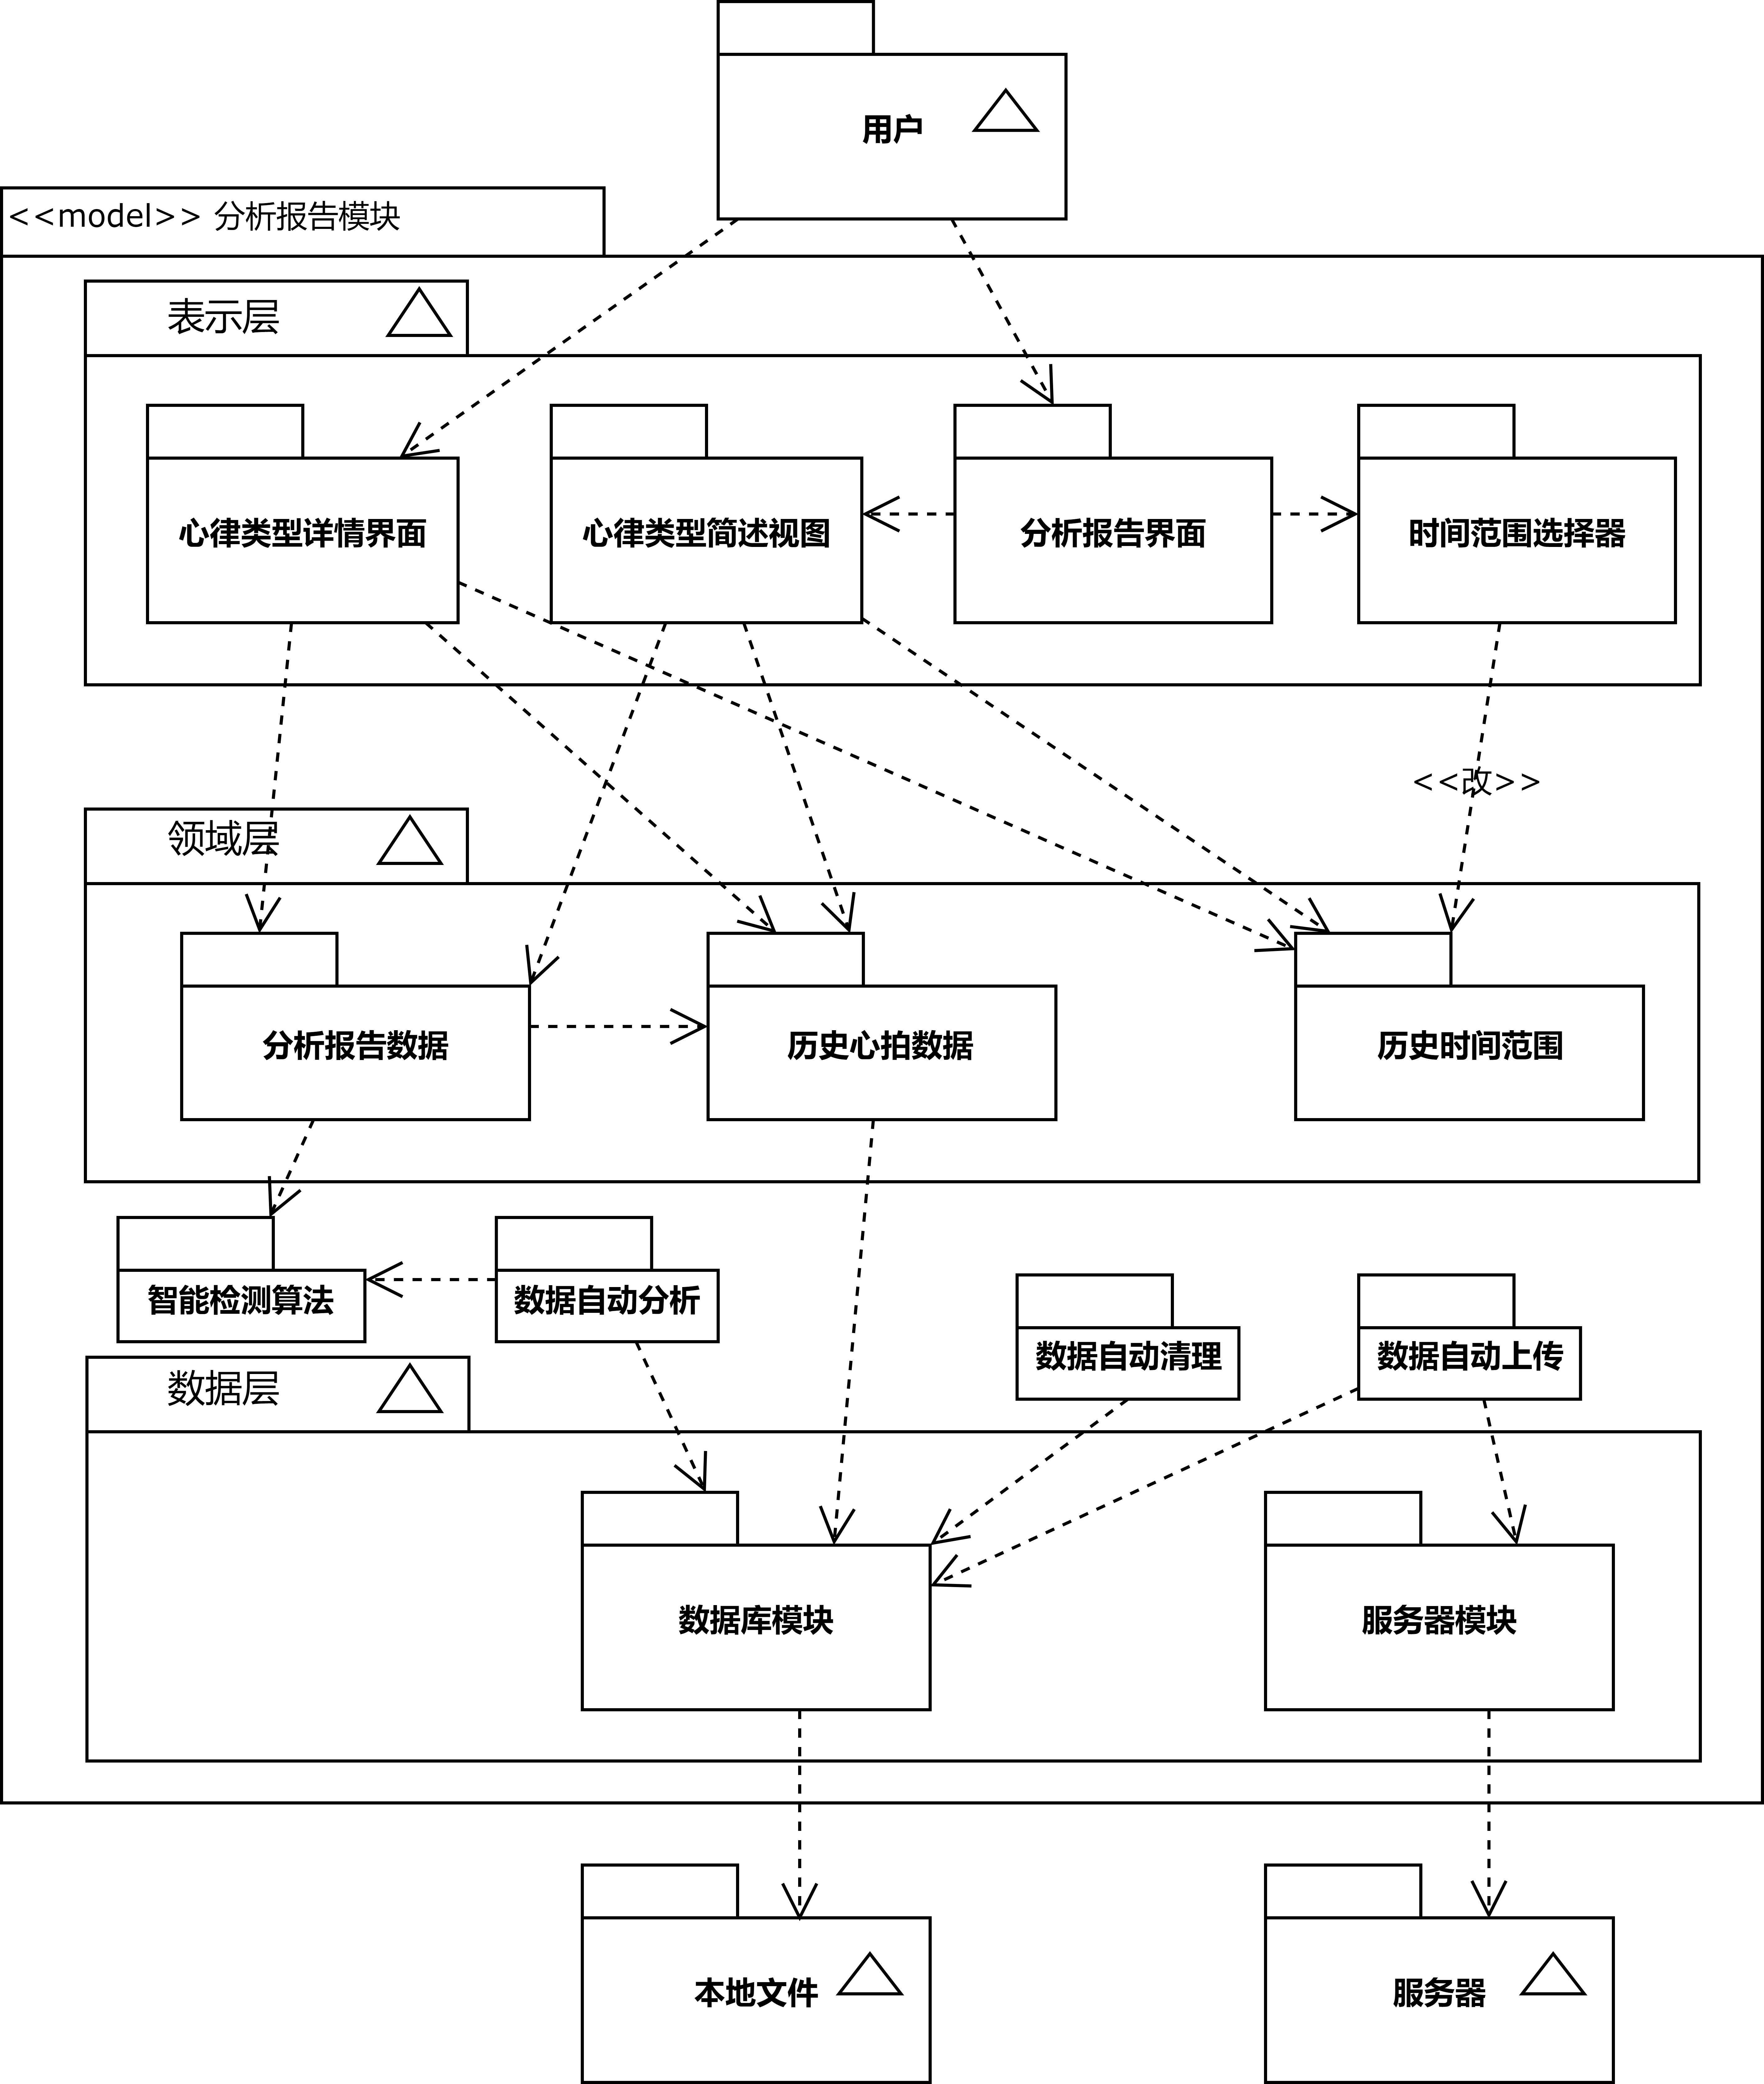
\includegraphics[width=.8\textwidth]{../assets/model-analytics.drawio}
    \bicaption{分析报告模块的架构}{Architecture of the analytics module}
    \label{fig:model-analytics}
\end{figure}

\subsubsection{表示层}

分析报告模块的表示层包含两个界面,分别是分析报告界面和心律类型详情界面。分析报告界面用于展示对各个心律类型的分析结果的总结,包含心律类型简述视图和用于控制分析时间段的时间范围选择器。点击某个心律类型简述视图所在区域后,会打开心律类型详情界面,详细说明该心律类型的情况,包括该心律类型每次出现的时间,点击时间可以跳转至历史心电界面的对应时间。

\subsubsection{领域层}

分析报告模块的领域层包含三个数据模型,分别是分析报告数据、历史心拍数据和历史时间范围。三个数据都同时被心律类型简述视图和心律类型详情界面所读取,因为前者只是后者的折叠形式。历史时间范围还被时间范围选择器展示和设置。历史时间范围即当前所查看的分析报告包含的时间范围,被读取后用于历史心拍数据的查询参数。历史心拍数据即过去的每个心拍的位置和对应的心律类型。分析报告数据是基于历史心拍数据的分析结果,比如平均心室率等。

\subsubsection{其他层}

数据自动清理模块和数据自动上传模块与历史心电中的作用相同,不进行重复说明。数据自动分析模块每10分钟自动运行一次(这是所用模型允许的最短输入数据的时长),读取过去10分钟的历史心电数据,输入智能检测算法,将得到的心拍分类结果写入数据库。该算法在后台自动运行,而非延迟到用户查询分析报告时再运行,原因之一是为了能将分析结果及时上传至服务器;原因之二是分析每10分钟的数据需要数秒时间,虽然不长,但用户选取较长范围时仍需要一定时间的等待,提前分析并存入数据库可以作为缓存;原因之三是历史心拍数据比较容易裁切和拼接,方便分段存入数据库和进行任意时间段的查询。而基于历史心拍数据分析得到的分析报告数据则因为计算量小而没有必要预先缓存,且较难进行多时间段的拼接和分离,因此在用户查询分析报告时才进行分析。

\subsubsection{数据层}

分析报告模块需要用到数据层中的数据库模块和服务器模块。数据库模块用于历史心电数据的查询、历史心拍数据的写入与查询。服务器模块用于数据上传。心电设备模块在分析报告模块中并不需要,用户甚至可以在已经断开心电监测设备的连接时查看分析报告,并不会对本模块的功能产生影响。

\subsection{设备管理模块的设计}\label{subsec:device-design}

设备管理模块的整体架构如图~\ref{fig:model-device} 所示。

\begin{figure}[!ht]
    \centering
    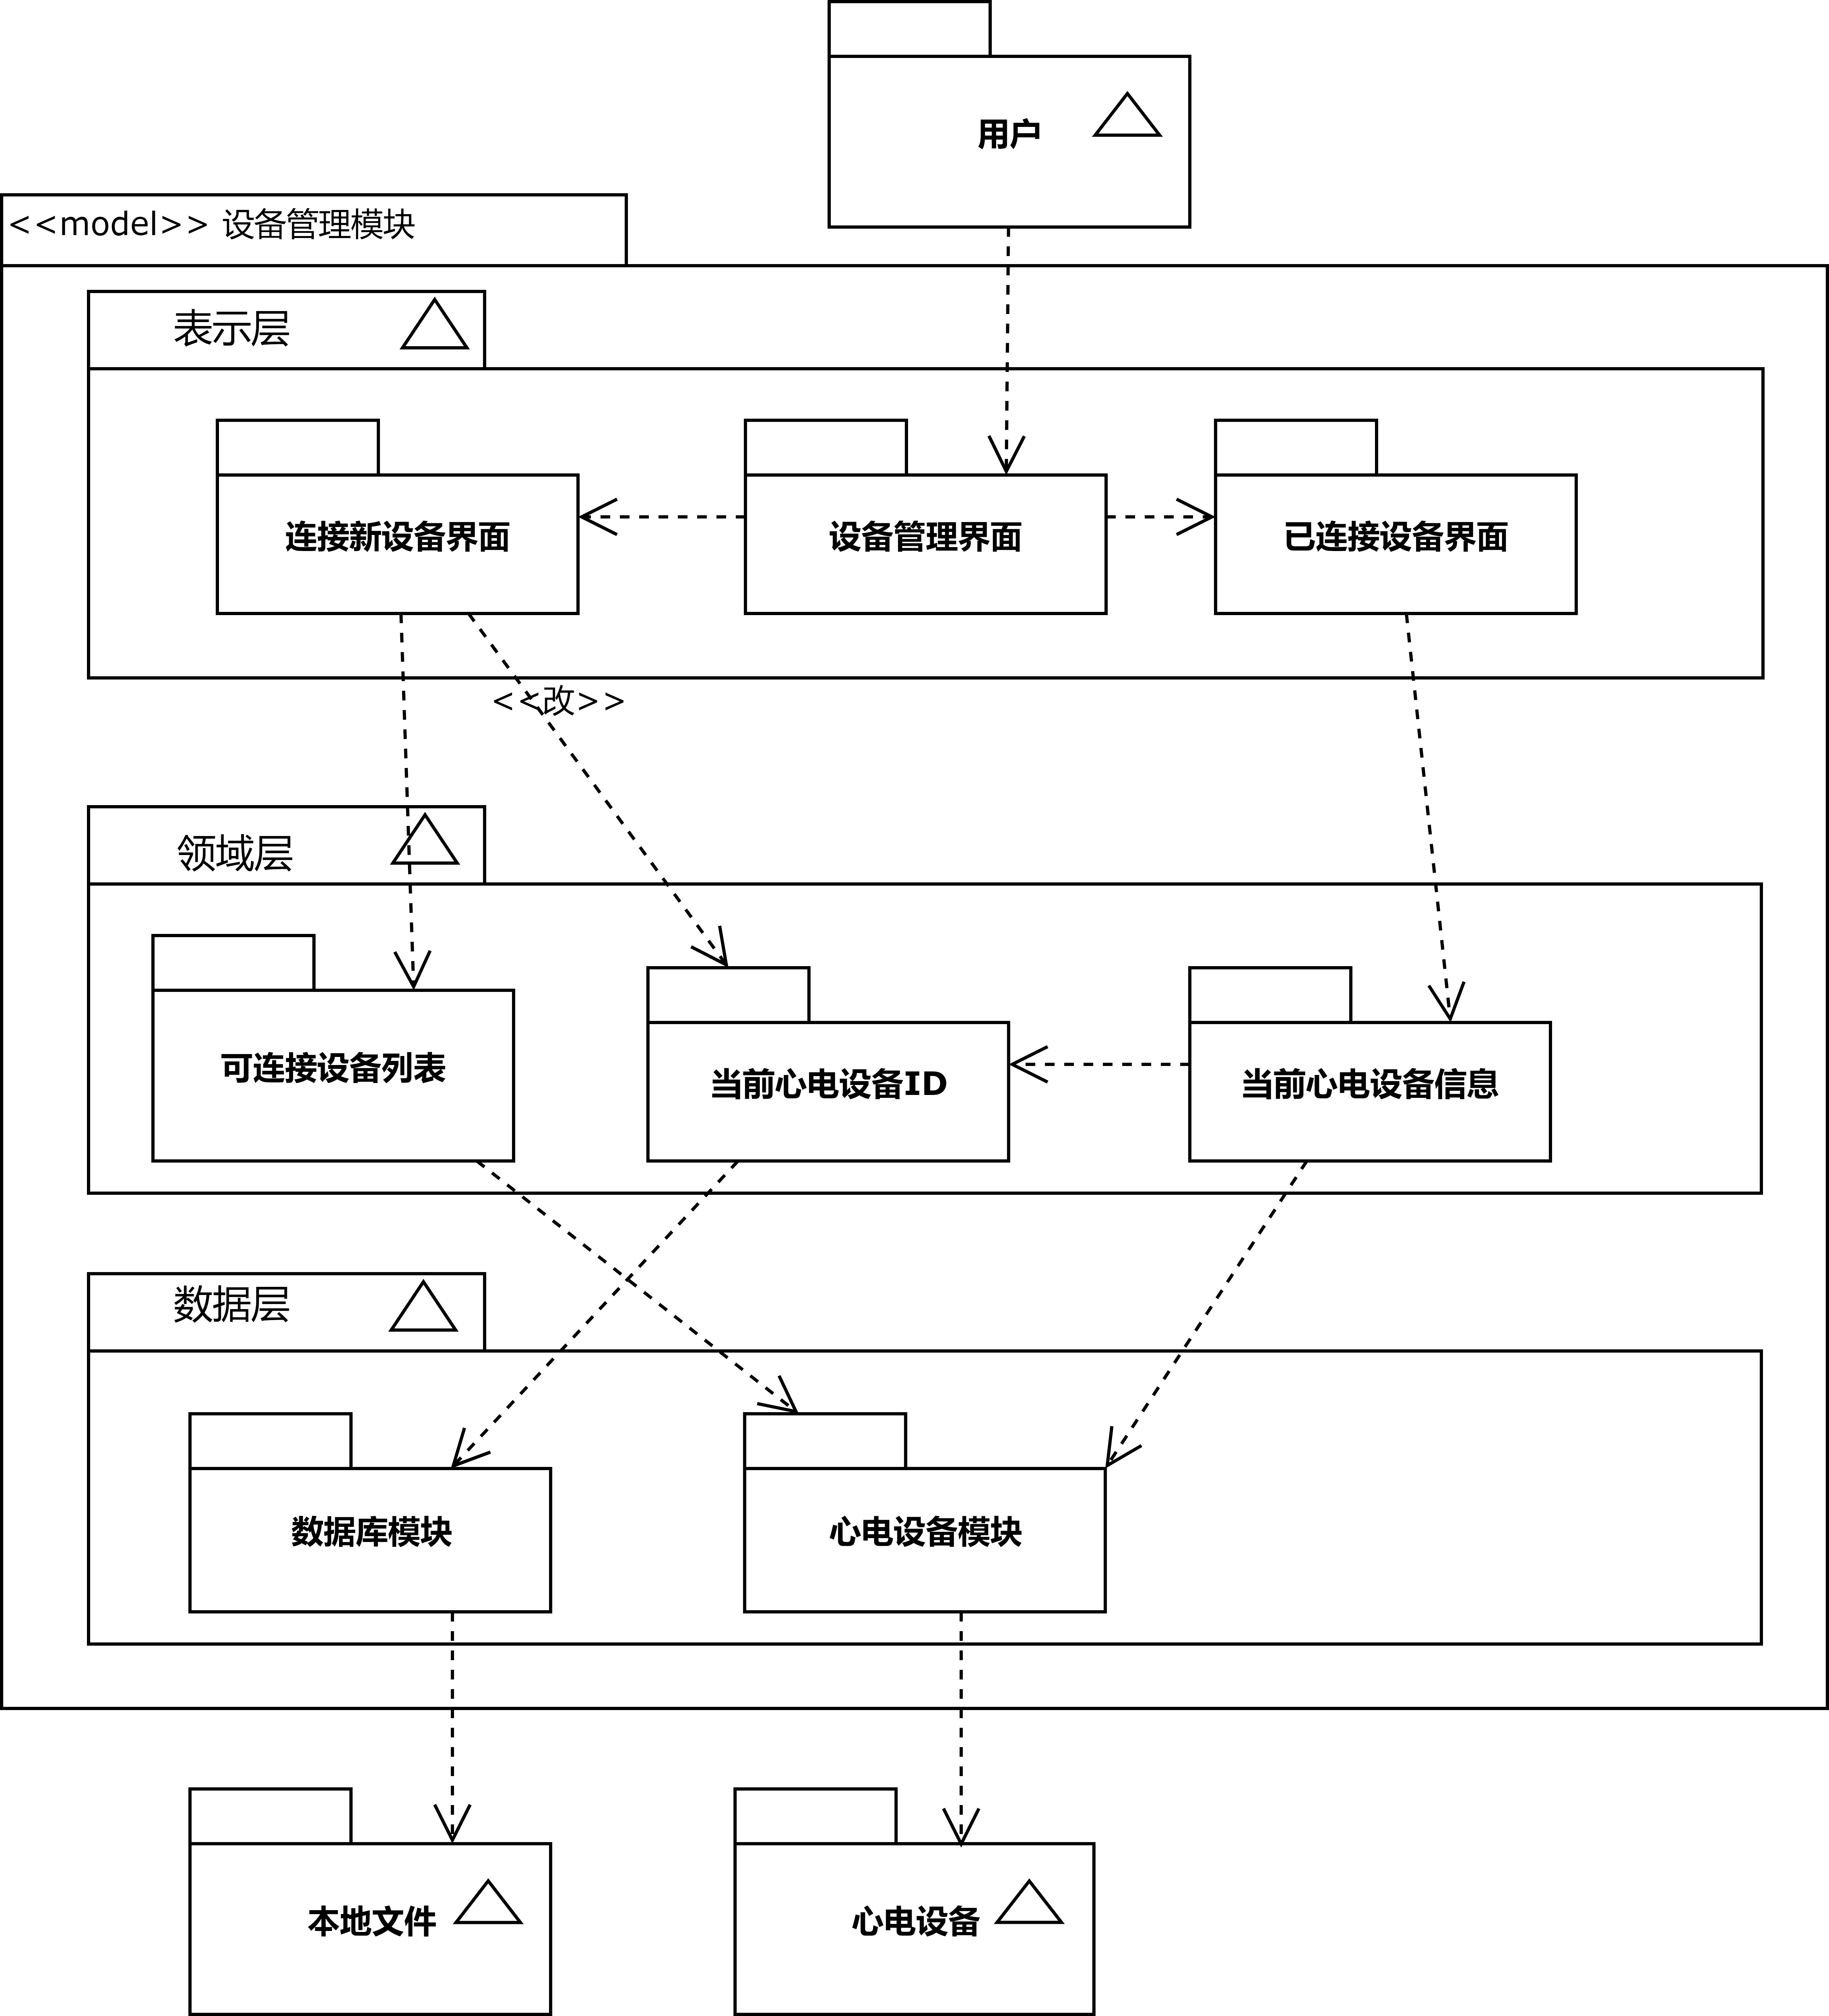
\includegraphics[width=.9\textwidth]{../assets/model-device.drawio}
    \bicaption{设备管理模块的架构}{Architecture of the device module}
    \label{fig:model-device}
\end{figure}

\subsubsection{表示层}

设备管理模块相比上述模块较为简单。虽然还有其他更简单的模块(如日志模块等),但因为在设计阶段几乎没有相关工作,故其他模块不在此章介绍。设备管理模块的表示层只包含一个面向用户的界面,即设备管理界面。设备管理界面实际上由两个不同的界面组成,在未连接设备的情况下是连接新设备界面,已连接设备的情况下则是已连接设备界面。由于两个界面的出现条件对立,因此将其合并为设备管理界面。在已连接设备界面中,点击解绑设备则会断开连接,切换至连接新设备界面。在连接新设备界面中,选择要连接的新设备则会进行连接,切换至已连接设备界面。

\subsubsection{领域层}

设备管理模块的领域层包含三个数据模型,即可连接设备列表、当前心电设备ID、当前心电设备信息。当前心电设备ID为字符串或 @null@,用于标识应用当前连接的设备,在应用程序启动时会从数据库读取,改变时也会写入数据库,设备管理界面在连接新设备界面和已连接设备界面之间的切换判定也是基于当前心电设备ID是否为 @null@。当前心电设备信息仅在心电设备已连接,即当前心电设备ID不为 @null@ 时有效,由已连接设备界面使用,其内容包括当前设备的信号强度、剩余电量等信息。可连接设备列表仅在连接新设备界面中有使用,为其提供可连接设备的名称与ID等信息,在连接后也会将所连接设备的ID更新至当前心电设备ID。

\subsubsection{数据层}

设备管理模块需要用到数据层中的数据库模块和心电设备模块。数据库模块用于连接的心电设备的ID的读写。心电设备模块用于与心电设备的通信和可供连接的设备的扫描。


\section{应用的数据库设计}\label{sec:db-design}

应用的数据库分为两部分,存储简单数据的SharedPreferences数据库和存储复杂数据的Isar数据库。前者主要用于存储应用的设置,后者主要用于存储历史心电数据与分析报告结果。

\subsection{SharedPreferences数据库的设计}\label{subsec:shared-preferences}

\subsubsection{SharedPreferences数据库介绍}\label{subsubsec:shared-preferences-intro}

SharedPreferences是Flutter的一个包,提供了简单键值对的存储功能,可以视为一个键值型的非关系型数据库。其在Android平台上基于同名的SharedPreferences功能,在iOS上则基于NSUserDefaults功能。

SharedPreferences仅支持少数几种数据类型,即 @int@、@double@、@bool@、@String@ 以及 @List<String>@。键值型数据库的读写非常简单,不需要进行特别的设计。本项目对该数据库的设计主要在于将各种需要存储的类型映射为其支持的类型。

\subsubsection{Duration类型的存储}\label{subsubsec:duration-storage}

Duration类型表示时间长度。由于应用内对时间的各种操作最多只需要毫秒精度,所以应用在需要将Duration类型的数据存入SharedPreferences时会将其转换为毫秒数以整数格式进行存储。在读取时,应用会将毫秒数转换为Duration类型。

\subsubsection{Color类型的存储}\label{subsubsec:color-storage}

Color类型表示颜色。应用在需要将Color类型的数据存入SharedPreferences时,会将其编码为32位整数以整数格式进行存储。在读取时,应用会将32位整数转换为Color类型。具体的编码方式是将颜色的ARGB值分别存储在32位整数的高8位、次高8位、次低8位和低8位中。

\subsubsection{枚举类型的存储}\label{subsubsec:enum-storage}

应用中使用了各种枚举类型,有时会需要将枚举类型存入SharedPreferences。应用在存储枚举类型时会将其转换为索引值,以整数形式存储。枚举类型常见的存储方式还包括按其名称以字符串形式存储、为每个枚举值赋予自定义值然后按自定义值的类型存储。相比其他方法,直接按索引值存储的优点在于其简单高效;缺点在于已经存在的枚举值不能轻易改动,否则会破坏已有的数据。由于应用内的枚举值设计基本不变,所以该缺点并不明显,可以接受。

\subsection{Isar数据库的设计}\label{subsec:isar}

\subsubsection{Isar数据库介绍}\label{subsubsec:isar-intro}

Isar是Flutter的一个包,提供了一个跨平台数据库。Isar属于非关系型数据库,不过提供了组合索引、ACID语义、事务等功能,可以视为一个关系型数据库的子集。相比常规的关系型数据库,Isar有一些额外的限制(或者说缺少一些功能)影响了本应用对数据库的设计。

当使用Isar来存储数据时,需要对Collection进行操作。Collection可理解为Isar数据库中的表,其包含的数据只能为同一类Dart对象,每个对象则代表了对应数据表中的一行数据。该类对象所对应的类则是这张表的Schema,其中每个字段对应数据库中的一列。与一般的关系型数据库相同的是,Schema中必须要有主键;不同的是,Isar中主键的类型被限制为64位整数值,这一限制导致了本应用对数据库的设计中的一些不同之处。

在查询时,Isar并不像一般的关系型数据库那样在编写SQL语句后自动生成最优查询策略,而是需要手动指定查询方式。Isar中的查询过滤方式分为两种,分别称为Filter和Where,前者执行遍历过滤,后者依靠索引表进行过滤。多个Where子句的过滤结果直接只能进行并集运算,无法进行交集运算。如果需要按多个属性进行过滤,并且还希望使用索引加快速度,就必须使用组合索引。组合索引有一个特殊的限制:主键不能包含在组合索引之中。这一限制也影响了本应用对数据库的设计。

此外,Isar对外键、Join等功能的支持也比较有限,不过这些功能在本应用的数据库设计中本来也不需要,所以不进行过多说明。

\subsubsection{心拍数据的存储}\label{subsubsec:beat-storage}

在分析报告数据中,只有心拍数据被存入数据库,基于心拍数据产生的进一步分析结果则只在查询时动态生成。这一方面是因为算法的大部分时间开销在于分割分类模型的运行上,其余部分开销较小。另一方面是因为心拍之外的结果的格式较为复杂,不方便进行合适的数据库设计。心拍数据则格式简单,且存储、查询时可以对多段数据进行拼接、裁剪而不失去太多准确度,所以适合存入数据库之中。

心拍数据的Schema包含3个字段和2个索引。字段中的ID是由Isar管理的自增整数,没有特别用途。另外两个字段分别是DateTime类型的心拍时间和枚举类型的心拍类型标签。对心拍时间进行了单列索引,以方便在查看历史心电时快速检索指定时间范围内的所有心拍。对心拍类型和心拍时间进行了组合索引,以心拍类型为主索引,这个组合索引用于查询指定标签在指定时间范围内的数量等信息。

\subsubsection{心电数据的存储}\label{subsubsec:point-storage}

对心电数据的查询需求较为简单,只有在历史心电界面中需要对指定时间范围内的心电数据进行查询。因此,也只需要在心电数据的时间上进行索引。

由于没有组合索引的需求,所以可以直接把时间作为主键,以节省额外的索引表的开销,并避免浪费主键所占的空间。由于主键只能为64位整数,所以需要对时间进行编码。考虑到时间只需要毫秒精度,将其编码为了自Unix纪元(UTC时间的1970年1月1日00:00:00)以来经过的毫秒数。这样,心电数据的Schema中不包含任何额外定义的索引,查询时只使用主键自带的索引功能。

除了作为主键的时间之外,一条心电数据中还包含各导联的电压数据。由于导联I、II、III被定义为左臂、右臂、左腿三个点之间的电位差,这三个导联的数据实际上只包含两个差值的信息量,所以只需要存储两个值即可。

    \chapter{\app 的开发}\label{ch:dev}

\todo{系统开发环境与开发工具}
\todo{本地}
\todo{持续集成}

\todo{系统功能实现}

    \documentclass[printMode]{ecnuthesis}
% 模版选项:
% printMode     是否开启打印模式, 若缺省则为关闭, 反之则为开启
% 用法示例
% \documentclass[printMode]{ecnuthesis}   (开启打印模式, 适合双面打印)
% \documentclass{ecnuthesis}              (关闭打印模式, 适合提交电子版)

\ecnuSetup {
  % 参数设置
  % 允许采用两种方式设置选项:
  %   1. style/... = ...
  %   2. style = { ... = ... } 
  % 注意事项: 
  %   1. 请勿在参数设置中出现空行
  %   2. "=" 两侧的空格将被忽略
  %   3. "/" 两侧的空格不会被忽略
  %   4. 请使用英文逗号 "," 分隔选项
  %
  % info 类用于输入论文信息
  info = {
    title = {基于微信小程序的线下课程考勤系统的设计与实现},
    % 中文标题
    %
    titleEN = {Design and Implementation of Offline Course Attendance System Based on WeChat Mini Program},
    % 英文标题
    %
    author = {张三},
    % 作者姓名
    %
    studentID = {10000000000},
    % 作者学号
    %
    department = {理工学院},
    % 学院名称
    %
    major = {计算机科学与技术},
    % 专业名称
    %
    supervisor = {李四},
    % 指导教师姓名
    %
    academicTitle = {教授},
    % 指导教师职称
    %
    year  = 2077,
    % 论文完成年份
    %
    month = 5,
    % 论文完成月份
    %
    keywords = {微信小程序, 课堂考勤, Java 语言, My Sql 数据库},
    % 中文关键词
    % 请使用英文逗号 "," 以分隔
    %
    keywordsEN = {WeChat Mini Program, Class attendance, Java, My Sql},
    % 英文关键词
    % 请使用英文逗号 "," 以分隔
    %
  },
  % style 类用于简单设置论文格式
  style = {
    footnote  = plain,
    % 脚注编号样式
    % 可用选项:
    %   footnote = plain|circled
    % 说明:
    %   plain     脚注的编号仅为数字
    %   circled   脚注的编号为带圆圈数字 (仅限1-10)
    %   (默认选项为 plain )
    %
    numbering = arabic,
    % 章节编号样式
    % 可用选项:
    %   numbering = arabic|alpha|chinese
    % 说明:
    %   arabic    使用数字进行编号 (即理科要求)
    %   alpha     使用字母进行编号 (即外文要求)
    %   chinese   使用汉字进行编号 (即文科要求)
    %   (默认选项为 arabic )
    %
    fontCJK = windows,
    % 中文字体选择
    % 可用选项:
    %   fontCJK = fandol|windows|mac
    % 说明:
    %   fandol    使用 TeX 自带的 fandol 字体
    %   windows   使用 Windows 系统内的字体 (中易)
    %   mac       使用 MacOS 系统内的字体
    %   (默认选项为 fandol )
    %
    fontMath = lm,
    % 数学字体选择
    % 可用选项:
    %   fontMath = lm|times
    % 说明:
    %   lm        使用 TeX 自带的 Latin Modern 数学字体
    %   times     使用 Times 风格的数学字体
    %   (默认选项为 lm )
    %
    bibResource = {./source/thesis-ref.bib},
    % 参考文献数据源
    % 由于使用的是 biber + biblatex , 所以必须明确给出 .bib 后缀名
    %
    logoResource = {./source/inner-cover(contains_font).eps},
    % 封面插图数据源
    % 模版已自带, 位于 ./source/inner-cover(contains_font).eps
    % 默认值为空
  }
}

% 需要的宏包可以自行调用
\usepackage{mwe}

\begin{document}

% 设置前置部分编号
\frontmatter

% 中文摘要环境
\begin{abstract}
  针对传统的课堂点名方式不仅浪费宝贵的时间,而且加重了教师的工作量。因此,借助微信平台为入口,基于微信小程序建立一个课堂考勤系统。文章采用 Java 语言编写,用 Spring Boot 框架实现,选择 My Sql 作为后台数据库,前端用微信开发工具开发,后台使用 Intelli J idea,在降低系统成本的同时并未降低系统的稳定性和可靠性。基于微信小程序开发的课堂考勤系统可以大大节省了课堂和教师的时间成本,并且该系统开发周期短,软件升级维护方便。实测结果表明,本系统运行稳定可靠,达到了快速组建班级、签到、请假等要求。
\end{abstract}

% 英文摘要环境
\begin{abstractEN}
  The traditional classroom roll call not only wastes precious time, but also increases the workload of teachers. Therefore, with the help of the WeChat platform as the entrance, a classroom attendance system based on the WeChat applet is established. The article is written in Java language and implemented with the Spring Boot framework. My Sql is selected as the back-end database, the front-end is developed with WeChat development tools, and the back-end uses Intelli J idea, which reduces the system cost while not reducing the stability and reliability of the system. The classroom attendance system developed based on the WeChat applet can greatly save the time cost of the classroom and teachers, and the system development cycle is short, and the software upgrade and maintenance are convenient. The actual test results show that the system runs stably and reliably, and meets the requirements of rapid class formation, sign-in, and leave.
\end{abstractEN}

% 设置正文编号
\mainmatter

\chapter{绪论}
\section{背景}
\subsection{浅谈中国软件}
\subsubsection{简介}

大字版手机银行、加粗版汇款界面、语音版绑卡流程、刷存折取款ATM机具……随着国务院办公厅《关于切实解决老年人运用智能技术困难的实施方案》的印发,当前金融服务领域已有多项“适老”措施有序推进。

\paragraph{国际性站点支撑}

其中关键问题在于如何把准老年人的切实需求,也就是说,老年人究竟需要什么样的金融服务?只有强化问题导向和需求导向,才能有效解决老年人的难题,保证各项措施落地见效。

\begin{theorem}[素数定理]
  设$x \geqslant 1$, 记$\pi(x)$表示不超过$x$的素数的个数, 则当$x \to \infty$时成立
  \[\pi(x) \sim \frac{x}{\ln x}\]
\end{theorem}

\begin{proof}
  是的,以上很多步骤在当时看起来非常的不严谨,但想不到后人通过严格的数学证明,发现它居然真的是对的。有的时候数学研究,不一定非要局限于你所在的领域,有时也可以先大胆的思考、尝试,然后再回过头来补全它,不要因为害怕而限制住了自己的思维。
  \[\pi(x) \sim \frac{x}{\ln x}\]
  命题得证。
\end{proof}

记者近日走访北京市多家银行网点、大型商超\footnote{商超指超市}、菜市场等老年人高频消费场所后发现,由于老年人所处的年龄段、教育背景、生活习惯不同,其金融服务需求也存在较大差异,因此需要分类施策,采取有针对性、差异性的解决方案。

\begin{lstlisting}[language=C++]
#include <stdio.h>
int main(int argc, char **argv) {
    printf("Hello world!\n");
    return 0;
}
\end{lstlisting}

根据记者的调查结果,老年人的金融服务需求总体可分为三类,分别对应三个不同年龄段。一是刚刚退休的人群,年龄集中在55岁至60岁;二是\footnote{帝鸿指黄帝帝鸿指黄帝帝鸿指黄帝帝鸿指黄帝帝鸿指黄帝帝鸿指黄帝帝鸿指黄帝帝鸿指黄帝帝鸿指黄帝帝鸿指黄帝帝鸿指黄帝帝鸿指黄帝帝鸿指黄帝帝鸿指黄帝帝鸿指黄帝帝鸿指黄帝帝鸿指黄帝帝鸿指黄帝帝鸿指黄帝帝鸿指黄帝}退休10年以内的人群,年龄集中在60岁至70岁;三是退休10年以上的人群,年龄多在70岁以上,有些甚至已进入耄耋之年。\footnote{【正义】:一本云“天下之民,谓之浑沌.”}

“我使用手机银行快10年了,不觉得自己比年轻人用得差。”家住北京市海淀区北太平庄街道的于女士笑称,她今年58岁,已退休3年多,还在岗位时银行卡、手机银行已发展多年。“我40多岁时用银行卡,后来接触手机银行并尝试网购,因为当时年纪相对较轻,学起来容易上手。”

\[
  \lim_{p\to+\infty}\int_{a}^{b}f(x)\sin{px}\,\mathrm{d}x = 0.
\]

尽管手机银行使用熟练,但办理大额资金交易时,这些老年人仍青睐线下渠道。为什么不选择线上渠道?于女士说,一是线上渠道不支持大额转账,二是线上渠道“不安全”,针对老年人的电信诈骗频发。实际上,据记者了解目前各家商业银行均已支持线上大额资金转账,用户拨打银行电话客服即可调整转账限额。

由此可见,除了“信息不对称”因素,制约这类老年人运用智能技术的梗阻还在于外部环境的安全性。因此,解决“不敢用”问题迫在眉睫。国务院此前已召开打击治理电信网络新型违法犯罪工作部际联席会议,部署全国“断卡”行动,严厉打击、整治非法开办贩卖电话卡、银行卡等违法行为,铲除电信网络诈骗案件滋生的土壤。据统计,2020年前10月,全国共破获电信网络诈骗案件15.5万起,同比上升65.6%;拦截处置诈骗电话5100万余次、诈骗短信6.3亿余条,成功止付冻结涉案资金1000余亿元。

这几天心里颇不宁静。今晚在院子里坐着乘凉,忽然想起日日走过的荷塘,在这满月的光里,总该另有一番样子吧。月亮渐渐地升高了,墙外马路上孩子们的欢笑,已经听不见了;妻在屋里拍着闰儿,迷迷糊糊地哼着眠歌。我悄悄地披了大衫,带上门出去。

沿着荷塘,是一条曲折的小煤屑路。这是一条幽僻的路;白天也少人走,夜晚更加寂寞。荷塘四面,长着许多树,蓊蓊郁郁的。路的一旁,是些杨柳,和一些不知道名字的树。没有月光的晚上,这路上阴森森的,有些怕人。今晚却很好,虽然月光也还是淡淡的。

路上只我一个人,背着手踱着。这一片天地好像是我的;我也像超出了平常的自己,到了另一世界里。我爱热闹,也爱冷静;爱群居,也爱独处。像今晚上,一个人在这苍茫的月下,什么都可以想,什么都可以不想,便觉是个自由的人。白天里一定要做的事,一定要说的话,现在都可不理。这是独处的妙处,我且受用这无边的荷香月色好了。

曲曲折折的荷塘上面,弥望的是田田的叶子。\footnote{很牛逼}叶子出水很高,像亭亭的舞女的裙。层层的叶子中间,零星地点缀着些白花,有袅娜地开着的,有羞涩地打着朵儿的;正如一粒粒的明珠,又如碧天里的星星,又如刚出浴的美人。微风过处,送来缕缕清香,仿佛远处高楼上渺茫的歌声似的。这时候叶子与花也有一丝的颤动,像闪电般,霎时传过荷塘的那边去了。叶子本是肩并肩密密地挨着,这便宛然有了一道凝碧的波痕。叶子底下是脉脉的流水,遮住了,不能见一些颜色;而叶子却更见风致了。

月光如流水一般,静静地泻在这一片叶子和花上。薄薄的青雾浮起在荷塘里。叶子和花仿佛在牛乳中洗过一样;又像笼着轻纱的梦。虽然是满月,天上却有一层淡淡的云,所以不能朗照;但我以为这恰是到了好处——酣眠固不可少,小睡也别有风味的。月光是隔了树照过来的,高处丛生的灌木,落下参差的斑驳的黑影,峭楞楞如鬼一般;弯弯的杨柳的稀疏的倩影,却又像是画在荷叶上。塘中的月色并不均匀;但光与影有着和谐的旋律,如梵婀玲上奏着的名曲。

荷塘的四面,远远近近,高高低低都是树,而杨柳最多。这些树将一片荷塘重重围住;只在小路一旁,漏着几段空隙,像是特为月光留下的。树色一例是阴阴的,乍看像一团烟雾;但杨柳的丰姿,便在烟雾里也辨得出。树梢上隐隐约约的是一带远山,只有些大意罢了。树缝里也漏着一两点路灯光,没精打采的,是渴睡人的眼。这时候最热闹的,要数树上的蝉声与水里的蛙声;但热闹是它们的,我什么也没有。

\chapter{忘了}

对于退休10年以内的人群,他们的金融需求有何特点?阻碍他们获取金融服务的“堵点”是什么?记者调查发现,这一群体可细分为两类,一类接受新技术的意愿、能力较强,其金融服务需求与刚退休人群相似;另一类有潜在的智能技术运用需求,如果有人帮助,他们愿意尝试。

在中国工商银行北京广安门支行营业室,上午9点开门后就有老年人陆续前来办理业务。“等待中的老年客户有时会问,为什么排在我后面的那位老人提前走了?他办完业务了吗?这时我们会告诉他,那位老人是通过自助机具办的业务,所以更快,进而询问他是否愿意尝试。”中国工商银行北京广安门支行营业室主任张然说,在银行工作人员的引导与帮助下,不少老年客户对智能服务积极接受,也认可其便捷性与安全性。

但受访老人普遍表示,如果身边没有专业人员指导,自己不会尝试独自使用智能机具,“不会用”“看不清”“怕出错”是主要顾虑。

如何解决以上问题?《实施方案》中明确提出,要推动金融机构、非银行支付机构等优化用户注册、银行卡绑定和支付流程,打造大字版、语音版、简洁版等“适老”手机银行。

“如果手机银行系统识别出客户的年龄在55岁以上,会将常用功能自动切换为老年版。”工商银行相关负责人表示,该行已针对老年群体推出手机银行“幸福生活版”,目前用户数已超1300万。

与标准版相比,老年版手机银行在字号、推荐模块等方面均有不同。记者看到,除页面字号增大外,功能页面中对重点信息的字号作了加大、加粗处理。例如在转账汇款界面,用户输入金额后会弹出对话框,里面显示的是放大后的数字,汇款人姓名也会加粗显示,以便老人识别。

“关注老年客户使用需求是银行应尽的责任,希望能够让老年客户体会到金融智能服务的便捷与安全。”工行上述负责人说,该行老年版手机银行还新增了“安全向导”功能,引导老年客户主动使用“账户安全锁”“转账汇款预警”等智能风险控制服务。

对于退休10年以上甚至进入耄耋之年的老年人,他们的金融服务需求与以上两类人群有何不同?记者调查发现,银行卡、移动互联网技术普及时,上述老人大多已处于退休状态。他们对新技术的认知更为陌生,对传统手段更为依赖,不少人没有银行卡、坚持使用存折,且偏爱现金支付,极少使用移动支付手段。

“每个月15号、16号是发退休金的日子,我早晨会先去菜市场买菜,然后去银行取工资,再回家。”家住北京市西城区广安门外大街的宋先生今年79岁,因为不使用移动支付,拿着存折取现金便成为他“必须要完成的事”。当被问及是否愿意尝试银行卡、移动支付时,老人摆摆手说:“年纪越大越谨慎,存了一辈子钱,我看病、养老都靠它们啦,可不能出意外。”

\begin{figure}
    \centering
    \includegraphics[width=.5\textwidth]{example-image}
    \bicaption{对于退休10年以内的人群,他们的金融需求有何特点?阻碍他们获取金融服务的“堵点”是什么?}{For people who have retired within 10 years, what are the characteristics of their financial needs? What is the "blocking point" that prevents them from accessing financial services?}
  \end{figure}

“在鼓励推广新技术、新方式的同时,要强调保留老年人熟悉的传统服\footnote{摸了摸了摸了}务方式,我想这是一个硬性要求。”国家发展改革委秘书长赵辰昕说,《实施方案》中已明确提出,保留传统金融服务方式,任何单位和个人不得以格式条款、通知、声明、告示等方式拒收现金。

“人民币是我国法定货币,人民币现金是我国境内最基础的支付手段 \cite{Yang_Hy200215} ,任何单位和个人不得拒收。”中国人民银行科技司司长李伟说,央行会将“整治拒收现金工作”作为一项重点工作长期抓下去,强化日常监管,通过暗访巡查等多种方式开展摸底排查,同时建立违法主体名录库,重点跟踪、持续整治。

李伟表示,央行已从现金管理、支付服务、普惠金融三方面入手采取措施,旨在切实提升老年人日常金融服务的可得性和满意度。在普惠金融方面,接下来央行将指导金融机构聚焦老年人日常的高频金融场景,打造线上线下一体化、贴合老年人需求的“适老”金融服务。

% 正文后部分
\backmatter
% 导入参考文献 (需要通过 latexmk 编译后才能显示)
\PrintReference

% 附录环境
\begin{appendix}
  \chapter{杂物}
  感谢天,感谢地,感谢阳光照耀了大地。
\end{appendix}

% 致谢环境
\begin{acknowledgement}
  感谢天,感谢地,感谢阳光照耀了大地。
\end{acknowledgement}

\end{document}
    \chapter{总结与展望}\label{ch:conc}

\todo{总结与展望}


% 正文后部分
    \backmatter

    % 参考文献
    \PrintReference

    % \include 会导致这些不出现在目录,原因未知
    %! suppress = UnresolvedReference


\begin{appendix}

    \begingroup
    \renewcommand{\clearpage}{\relax}
    \listoftodos
    提到的网页链接应该放在脚注、参考文献,还是都不放?

    参考文献格式,国标和学校发的模板不一致,模板编译的结果只能按照 GB/T 7714—2015 标准(除非知道学校那个模板里是什么标准并找到对应的包)。一个可能的替代方案是完全确定参考文献后,用Word手动按学校模板格式打出来。
    \endgroup

    \listoffigures
    \listoffigureEng

\end{appendix}

    \begin{acknowledgement}

    (应盲审要求,隐去致谢内容。)

\end{acknowledgement}


\end{document}
